\documentclass[floatfix,aps,pra,twocolumn,superscriptaddress,10pt,nofootinbib]{revtex4-2}

\usepackage{graphicx}
\usepackage{bm}
\usepackage{booktabs}
\usepackage[title]{appendix}
\usepackage{float}
\usepackage{ragged2e}
\usepackage{amsmath,amssymb}
\usepackage{xcolor}
\usepackage{tikz}
\usepackage{hyperref}
\usetikzlibrary{arrows.meta,positioning,calc,decorations.pathreplacing,fit,backgrounds}


% ---------------------------------------------------------------------
% Colours used consistently in the figures: classical = blue, HQPINN (noiseless and on the real QPU) = orange,
% HQPINN on a noisy emulator = aqua. Fig. 3 is the exception, at the author's request: classical = black, one colour
% per width for the HQPINN.
\definecolor{qcol}{HTML}{EB6834}
\definecolor{ccol}{HTML}{2A78D6}
\definecolor{fcol}{HTML}{1BAF7A}

% Working notes -- set \showtodostrue -> \showtodosfalse to hide them all
\newif\ifshowtodos \showtodostrue
\newcommand{\TODO}[1]{\ifshowtodos\textcolor{red}{\textbf{[TODO:} #1\textbf{]}}\fi}

% Space reserved for a figure: \figspace{height}. The author asked to leave the inverse-problem plots out for now; to put one
% back, uncomment its \includegraphics line (the PDFs are still written by manuscript/scripts/) and delete the \figspace.
\newcommand{\figspace}[1]{\fbox{\parbox[c][#1][c]{0.97\textwidth}{\centering\small\color{gray!70!black}espa\c{c}o reservado para a figura}}}

\newtheorem{proposition}{Proposition}
\newtheorem{remark}{Remark}
\newcommand{\sg}{\operatorname{sg}}
\newcommand{\wmed}{\operatorname{wmed}}
\newcommand{\Ncol}{N_{\rm col}}

% Algorithms without extra packages: numbered, ruled, non-floating blocks
% (revtex4-2 and the float package's \newfloat do not combine)
\newcounter{algorithm}
\newenvironment{algorithm}[1]{\par\medskip\noindent\begin{minipage}{\linewidth}\refstepcounter{algorithm}%
  \hrule height 0.6pt\vspace{2pt}\noindent{\small\textbf{Algorithm~\thealgorithm.} #1}\vspace{2pt}\hrule height 0.3pt%
  \small\begin{list}{\arabic{enumi}:}{\usecounter{enumi}\setlength{\itemsep}{1pt}%
  \setlength{\parsep}{0pt}\setlength{\topsep}{3pt}\setlength{\leftmargin}{1.5em}\setlength{\labelwidth}{1.2em}}}%
  {\end{list}\vspace{2pt}\hrule height 0.6pt\end{minipage}\par\medskip}

\hypersetup{colorlinks=true, linkcolor=blue!50!black, citecolor=blue!50!black, urlcolor=blue!50!black}

\graphicspath{{figures/}}

\begin{document}

\title{Hybrid quantum physics-informed neural networks with a fixed quantum layer for forward and inverse problems}
% Alternative titles:
%  - "A non-variational quantum layer for physics-informed learning: forward and inverse problems, from simulation to a superconducting processor"
%  - "Training a physics-informed neural network with a fixed quantum layer on a superconducting quantum processor"

\author{Gubio G. de Lima}
\email{gubio.gomes@estudante.ufscar.br}
\affiliation{\TODO{afilia\c{c}\~ao (CBPF / UFSCar)}}

\author{Erick \TODO{sobrenome}}
\affiliation{\TODO{afilia\c{c}\~ao}}

\begin{abstract}
We study a physics-informed neural network whose middle block is a fixed quantum circuit with no trainable parameters, on the forward and inverse problems of the viscous Burgers equation. In the forward problem, with one common protocol and noiseless simulation, the hybrid model reaches the error of a classical network of the same form with about half of the optimizer steps and fewer parameters at the short horizon, and a lower error at the long horizon. Trained with a 120-qubit superconducting processor in the loop, with one job per epoch and no error mitigation, it reaches a relative error of 5.7\% in 110 epochs at the short horizon. In the inverse problem, with the quantum layer on a noisy emulator of the device, both models identify the viscosity with a median error below 3\% in 500 epochs at the short horizon, with no significant difference between them; at the long horizon neither identifies it accurately (median 21\% and 30\%), and the classical model reconstructs the field better in all cases. Since the noiseless layer is classically computable, the simulations measure the merit of an architecture, not a quantum advantage. \TODO{Rascunho do resumo. Faltam os resultados no QPU real: problema direto em $T=1$ e problema inverso nos dois $T$. Falta tamb\'em o problema inverso com 20\,000 \'epocas e circuito ideal, em que os dois modelos identificam $\nu$ em $T=1$ (mediana 3.1\% e 2.9\%).}
\end{abstract}

\maketitle

% =====================================================================
\section{Introduction}\label{sec:intro}
% =====================================================================
\TODO{Rascunho da introdu\c{c}\~ao, a revisar.}
Physics-informed neural networks (PINNs)~\cite{raissi2019physics,karniadakis2021physics} represent the solution of a partial differential equation (PDE) by a neural network trained on the residual of the equation. The same construction addresses two tasks: the \emph{forward} problem, in which the equation is known and its solution is sought, and the \emph{inverse} problem, in which an unknown parameter of the equation is learned together with the solution from sparse data~\cite{raissi2019physics}. Training a PINN is delicate at small collocation budgets and long time horizons~\cite{krishnapriyan2021characterizing,wang2021understanding,wang2022when}, which motivates the search for other functional forms of the network.

Quantum circuits have been proposed both as solvers of differential equations~\cite{lubasch2020variational,kyriienko2021solving,paine2023quantum} and as layers of hybrid PINNs~\cite{sedykh2024hybrid,berger2025trainable,farea2025qcpinn,lantigua2026classical,zabihi2026hybrid}. In these hybrid PINNs the circuit is trainable, which exposes the optimization to barren plateaus~\cite{mcclean2018barren,cerezo2021cost} and requires gradients of the device output, for example by parameter-shift rules~\cite{mitarai2018quantum,schuld2019evaluating}, and the results come from noiseless simulation. Fixed, non-variational quantum maps have been studied as feature maps~\cite{havlicek2019supervised}, reservoirs~\cite{fujii2017harnessing,mujal2021opportunities} and convolutional filters~\cite{henderson2020quanvolutional}, but not inside a physics-informed residual. To our knowledge, no PINN has been trained with a quantum processor in the loop. \TODO{confirmar as duas afirma\c{c}\~oes na revis\~ao bibliogr\'afica antes de submeter.} An obstacle is specific to this setting: the finite differences of the residual amplify the shot noise of the device.

Here we use a fixed quantum layer between two classical networks, and the same model and training machinery for both problems. All trainable parameters are classical. Since noise changes the coefficients of the layer but not its functional form, a calibrated classical surrogate of the device supplies the gradient and a noise-free interpolation across the finite-difference stencil, in a scheme analogous to physics-aware training of physical neural networks~\cite{wright2022deep}. In the inverse problem the viscosity enters the residual linearly and is updated in closed form by variable projection~\cite{golub1973differentiation}.

We report four sets of results for the viscous Burgers equation, against a classical PINN of the same form: the forward problem in simulation (Sec.~\ref{sec:f_sim}) and with the \texttt{ibm\_berlin} processor in the loop (Sec.~\ref{sec:f_qpu}), and the inverse problem in simulation with noisy emulators of the device (Sec.~\ref{sec:i_sim}) and on real hardware (Sec.~\ref{sec:i_qpu}, still pending). Because the noiseless layer is classically computable, the simulations measure the merit of an architecture rather than a quantum advantage~\cite{schreiber2023classical}. Section~\ref{sec:hqpinn} describes the model for both problems, Secs.~\ref{sec:forward} and~\ref{sec:inverse} give the results, and Secs.~\ref{sec:discussion} and~\ref{sec:conclusions} close the paper. The technical details of each of the four sets of results are in Appendices~\ref{app:fsim}, \ref{app:fqpu}, \ref{app:isim} and~\ref{app:iqpu}, respectively.

% =====================================================================
\section{Hybrid quantum PINN}\label{sec:hqpinn}
% =====================================================================
\subsection{Forward and inverse problems}\label{sec:problem}
We consider the viscous Burgers equation on the periodic unit interval,
\begin{equation}
  \partial_t u + u\,\partial_x u = \nu\,\partial_x^2 u,\qquad x\in[0,1),\ t\in[0,T],
  \label{eq:burgers}
\end{equation}
with $u(x,0)=\sin(2\pi x)$. Equation~\eqref{eq:burgers} is the simplest PDE that combines nonlinear advection with diffusion~\cite{basdevant1986spectral}. We use $\nu=0.01$ and two horizons. The inviscid solution breaks at $t=1/(2\pi)\simeq0.16$. At $T=0.1$ the profile has steepened ($\max_x|\partial_xu|\simeq13.6$, against $2\pi$ at $t=0$) but no shock has formed yet. At $T=1$ a viscous shock sits at $x=1/2$ and the wave has been strongly damped ($\max_xu$ drops from 0.96 at $T=0.1$ to 0.33, with $\|u\|_{\rm rms}\simeq0.21$), and the problem is harder.

In the \emph{forward problem} $\nu$ is known and $u$ is sought, with no solution data in the training. In the \emph{inverse problem} $\nu$ is unknown, and it is recovered together with $u$ from sparse observations
\begin{equation}
  \mathcal D=\{(x_i,t_i,u^\star_i)\}_{i=1}^{\Ncol},\qquad u^\star_i=u(x_i,t_i;\nu_{\rm true})+\varepsilon_i,
  \label{eq:data}
\end{equation}
here given by the exact solution (Appendix~\ref{app:colehopf}) with $\nu_{\rm true}=0.01$ and $\varepsilon_i=0$. This is a controlled first step towards the seismic inverse problem, in which a wave speed $c(x)$ plays the role of $\nu$. In both problems the residual of Eq.~\eqref{eq:burgers} is written as
\begin{equation}
  r=A-\nu\,B,\qquad A=\partial_tu+u\,\partial_xu,\qquad B=\partial_x^2u,
  \label{eq:residual}
\end{equation}
which makes explicit that $\nu$ enters linearly.

\subsection{Architecture}\label{sec:arch}
A PINN~\cite{raissi2019physics,karniadakis2021physics} represents the solution by a parametrized function $u_\Theta(x,t)$. Before entering the network, the inputs are mapped to the periodic feature vector $\bm\xi(x,t)=(\sin2\pi x,\cos2\pi x,t/T)$, so that periodicity is exact. The initial condition can be imposed in two ways. With a \emph{soft constraint} it enters the loss as a penalty, whose weight has to be balanced against the residual, a known source of training difficulties~\cite{wang2021understanding,krishnapriyan2021characterizing}. With a \emph{hard constraint} it is built into the form of the solution~\cite{lagaris1998artificial},
\begin{equation}
  u_\Theta(x,t)=\sin(2\pi x)+\frac{t}{T}\,\big(\mathcal N_{\rm post}\circ\mathcal M\circ\mathcal N_{\rm pre}\big)\big(\bm\xi(x,t)\big).
  \label{eq:composition}
\end{equation}
We use the hard constraint everywhere except in the inverse problem at $T=1$, where the soft constraint gave better results in training tests (Appendix~\ref{app:adjust}).

The classical pre-network $\mathcal N_{\rm pre}(\cdot;\bm\phi):\mathbb R^3\to\mathbb R^n$ maps the features to a latent vector $\bm\theta\in\mathbb R^n$, a middle block $\mathcal M:\mathbb R^n\to\mathbb R^n$ transforms it into $\bm y$, and the classical post-network $\mathcal N_{\rm post}(\cdot;\bm\psi):\mathbb R^n\to\mathbb R$ produces the output (Fig.~\ref{fig:schematic}). The middle block is the only part that distinguishes the two models compared here, and its size $n$ is the quantity we vary. In the \emph{classical PINN} it is a trainable network with one hidden layer of $m$ units,
\begin{equation}
  \mathcal M_{\rm C}(\bm\theta)=\mathcal N_{\rm mid}(\bm\theta;\bm\chi).
  \label{eq:bottleneck}
\end{equation}
In the \emph{hybrid quantum PINN} (HQPINN) it is a fixed quantum circuit: the latent vector is the set of rotation angles of $n$ qubits,
\begin{equation}
  \mathcal U(\bm\theta)=W_{\rm brick}\,\bigotimes_{q=1}^{n}R_Y(\theta_q),\qquad R_Y(\theta)=e^{-i\theta Y/2},
  \label{eq:circuit}
\end{equation}
where $W_{\rm brick}$ is one brickwork layer of nearest-neighbour CNOT gates, and the output is the vector of local magnetizations,
\begin{equation}
  \mathcal M_{\rm Q}(\bm\theta)=\bm y(\bm\theta),\qquad y_q(\bm\theta)=\operatorname{Tr}\!\big[Z_q\,\mathcal E_{\bm\theta}\big(|0\rangle\langle0|^{\otimes n}\big)\big],
  \label{eq:expval}
\end{equation}
where $\mathcal E_{\bm\theta}$ is the channel actually implemented by the device. On a device $y_q$ is estimated from $S$ shots.

\emph{The circuit has no free parameter}: all trainable parameters belong to the classical networks. The HQPINN has $21n+61$ trainable parameters. The classical PINN has $2nm+m+n$ more in its middle block: $2n^2+23n+61$ in total with $m=n$, used in the forward simulations, and $42n+71$ with $m=10$, used in the inverse problem and in the hardware-budget control. The two coincide at $n=10$, with 491 parameters against 271. This is the opposite design choice to the variational hybrid PINNs studied so far~\cite{sedykh2024hybrid,berger2025trainable,farea2025qcpinn,lantigua2026classical,zabihi2026hybrid}, and without trainable gates the barren-plateau phenomenon of variational circuits~\cite{mcclean2018barren,cerezo2021cost} does not arise.

\begin{figure*}[t]
  \centering
  \resizebox{\textwidth}{!}{% Fig. 1 -- classical PINN and hybrid quantum PINN (HQPINN): the architecture, general for the forward and inverse problems.
% \input inside a figure* (main.tex wraps it in \resizebox{\textwidth}{!}{...}).
% Needs the TikZ libraries arrows.meta, positioning, calc, decorations.pathreplacing, the package bm,
% and the colours qcol (HQPINN / QPU) and ccol (classical) defined in main.tex.
% Preview alone: see manuscript/figures/schematic_preview.tex
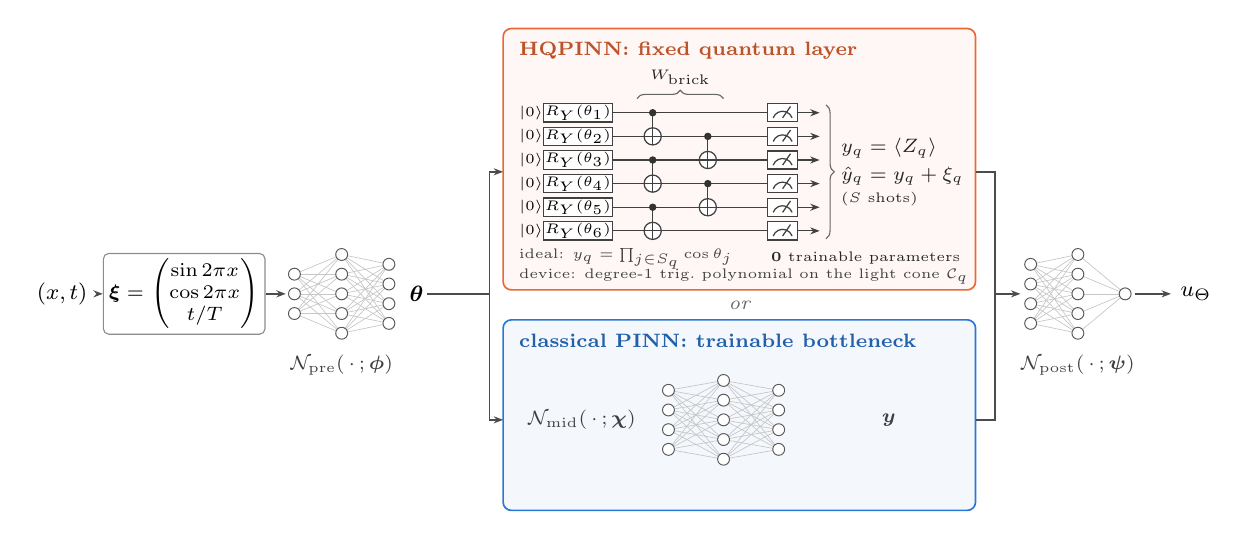
\begin{tikzpicture}[
  font=\footnotesize, >={Stealth[length=3.4pt]},
  arr/.style={->, line width=0.55pt, black!70},
  neuron/.style={circle, draw=black!65, fill=white, line width=0.35pt, inner sep=0pt, minimum size=4.3pt},
  wire/.style={black!75, line width=0.45pt},
  gate/.style={draw=black!75, fill=white, line width=0.45pt, inner sep=0.6pt, minimum height=0.23cm,
               minimum width=0.66cm, font=\tiny},
  note/.style={font=\scriptsize, black!75, align=center},
  tnote/.style={font=\tiny, black!75},
]
% ---- helpers: a column of neurons, all-to-all links between two columns, CNOT, meter
\def\ncol#1#2#3{\foreach \i in {1,...,#2}{\node[neuron] at (#1,{#3+(\i-(#2+1)/2)*0.25}) {};}}
\def\nlinks#1#2#3#4#5{\foreach \i in {1,...,#2}{\foreach \j in {1,...,#4}{%
  \draw[black!22, line width=0.25pt] (#1,{#5+(\i-(#2+1)/2)*0.25}) -- (#3,{#5+(\j-(#4+1)/2)*0.25});}}}
\def\cnot#1#2#3{\draw[wire] (#1,#2) -- (#1,#3); \fill[black!80] (#1,#2) circle (1.35pt);
  \draw[wire, fill=white] (#1,#3) circle (3.1pt);
  \draw[wire] ({#1-0.109},#3) -- ({#1+0.109},#3); \draw[wire] (#1,{#3-0.109}) -- (#1,{#3+0.109});}
\def\meter#1#2{\draw[wire, fill=white] ({#1-0.19},{#2-0.115}) rectangle ({#1+0.19},{#2+0.115});
  \draw[wire] ({#1-0.12},{#2-0.065}) arc (160:20:0.128); \draw[wire] (#1,{#2-0.065}) -- ({#1+0.1},{#2+0.08});}

% =====================================================================================
% shared classical pre/post networks, interchangeable middle block
% =====================================================================================
\node (in) at (0.45,2.75) {$(x,t)$};
\node[draw=black!45, rounded corners=2pt, fill=white, inner sep=2pt, font=\scriptsize, align=center] (xi) at (2.0,2.75)
  {$\bm\xi=\begin{pmatrix}\sin 2\pi x\\ \cos 2\pi x\\ t/T\end{pmatrix}$};
\draw[arr] (in) -- (xi);
% pre-network 3 -> 10 -> n
\nlinks{3.4}{3}{4.0}{5}{2.75}\nlinks{4.0}{5}{4.6}{4}{2.75}
\ncol{3.4}{3}{2.75}\ncol{4.0}{5}{2.75}\ncol{4.6}{4}{2.75}
\draw[arr] (xi.east) -- (3.29,2.75);
\node[note] at (4.0,1.85) {$\mathcal N_{\rm pre}(\,\cdot\,;\bm\phi)$};
\node[anchor=west, inner sep=1pt] (theta) at (4.82,2.75) {$\bm\theta$};
\coordinate (split) at (5.88,2.75);
\draw[line width=0.55pt, black!70] (theta.east) -- (split);

% ---- middle block, option 1: fixed quantum circuit (HQPINN)
\draw[qcol, line width=0.6pt, rounded corners=3pt, fill=qcol!5] (6.05,2.8) rectangle (12.05,6.12);
\node[anchor=north west, font=\scriptsize\bfseries, text=qcol!80!black] at (6.13,6.07) {HQPINN: fixed quantum layer};
\foreach \q/\y in {1/5.05,2/4.75,3/4.45,4/4.15,5/3.85,6/3.55}{
  \node[font=\tiny, anchor=east, inner sep=1pt] at (6.6,\y) {$|0\rangle$};
  \draw[wire] (6.6,\y) -- (9.41,\y);
  \node[gate] at (7.0,\y) {$R_Y(\theta_{\q})$};
  \meter{9.6}{\y}
  \draw[wire, ->] (9.79,\y) -- (10.07,\y);
}
\cnot{7.95}{5.05}{4.75}\cnot{7.95}{4.45}{4.15}\cnot{7.95}{3.85}{3.55}
\cnot{8.65}{4.75}{4.45}\cnot{8.65}{4.15}{3.85}
\draw[decorate, decoration={brace, amplitude=3pt}, black!60] (7.75,5.23) -- (8.85,5.23)
  node[midway, above=1.5pt, font=\tiny, black!85] {$W_{\rm brick}$};
\draw[decorate, decoration={brace, amplitude=3pt}, black!60] (10.15,5.15) -- (10.15,3.45)
  node[midway, right=2pt, font=\scriptsize, black!85, align=left]
  {$y_q=\langle Z_q\rangle$\\[2pt]$\hat y_q=y_q+\xi_q$\\[0pt]{\tiny ($S$ shots)}};
\node[tnote, anchor=west] at (6.13,3.2) {ideal: $y_q=\prod_{j\in S_q}\cos\theta_j$};
\node[tnote, anchor=west] at (6.13,2.97) {device: degree-1 trig.\ polynomial on the light cone $\mathcal C_q$};
\node[font=\tiny, anchor=east, black!85] at (11.98,3.2) {\textbf{0} trainable parameters};

% ---- middle block, option 2: trainable bottleneck (classical PINN)
\draw[ccol, line width=0.6pt, rounded corners=3pt, fill=ccol!5] (6.05,0.0) rectangle (12.05,2.42);
\node[anchor=north west, font=\scriptsize\bfseries, text=ccol!80!black] at (6.13,2.37) {classical PINN: trainable bottleneck};
\nlinks{8.15}{4}{8.85}{5}{1.15}\nlinks{8.85}{5}{9.55}{4}{1.15}
\ncol{8.15}{4}{1.15}\ncol{8.85}{5}{1.15}\ncol{9.55}{4}{1.15}
\node[note] at (7.05,1.15) {$\mathcal N_{\rm mid}(\,\cdot\,;\bm\chi)$};
\node[note] at (10.95,1.15) {$\bm y$};
\node[font=\scriptsize\itshape, black!60] at (9.05,2.61) {or};

% ---- routing theta -> middle block -> post-network
\draw[arr] (split) |- (6.05,4.3);
\draw[arr] (split) |- (6.05,1.15);
\draw[line width=0.55pt, black!70] (12.05,4.3) -- (12.3,4.3) -- (12.3,1.15) -- (12.05,1.15);
\draw[arr] (12.3,2.75) -- (12.62,2.75);
% post-network n -> 10 -> 1
\nlinks{12.75}{4}{13.35}{5}{2.75}\nlinks{13.35}{5}{13.95}{1}{2.75}
\ncol{12.75}{4}{2.75}\ncol{13.35}{5}{2.75}\ncol{13.95}{1}{2.75}
\node[note] at (13.35,1.85) {$\mathcal N_{\rm post}(\,\cdot\,;\bm\psi)$};
\node (u) at (14.85,2.75) {$u_\Theta$};
\draw[arr] (14.07,2.75) -- (u.west);

\end{tikzpicture}
}
  \caption{\justifying
  Classical PINN and hybrid quantum PINN (HQPINN). Both models share the classical pre-network $\mathcal N_{\rm pre}$, which maps the periodic features $\bm\xi$ to the latent vector $\bm\theta$, and the classical post-network $\mathcal N_{\rm post}$, which leads to the solution $u_\Theta$ [Eq.~\eqref{eq:composition}]. In the HQPINN (orange) the middle block is a \emph{fixed} quantum circuit---one $R_Y(\theta_q)$ rotation per qubit followed by one brickwork layer of CNOTs---whose output is the vector of local expectation values $y_q=\langle Z_q\rangle$, estimated with $S$ shots; the circuit has no trainable parameter. Six of the $n=10$ qubits used on hardware are drawn. In the classical PINN (blue) the middle block is a trainable bottleneck $\mathcal N_{\rm mid}$.}
  \label{fig:schematic}
\end{figure*}

\subsection{Physics-informed training}\label{sec:loss}
At every epoch $k$ a fresh batch of $\Ncol$ collocation points $(x_i,t_i)$ is drawn. The two problems share one form of the loss,
\begin{equation}
  \mathcal L_k(\Theta)=\frac{\rho_k}{\Ncol}\sum_{i} |r_i|^p+\frac{w_d}{\Ncol}\sum_{i}\big|u_\Theta(x_i,t_i)-u^\star_i\big|+w_0\,\mathcal L_{\rm ic},
  \label{eq:loss}
\end{equation}
with $r_i=r(x_i,t_i;\nu_k)$, and they differ in the terms that are switched on (Table~\ref{tab:problems}). The forward problem uses the squared residual alone ($p=2$, $\rho_k=1$, $w_d=w_0=0$), so that with the hard constraint Eq.~\eqref{eq:loss} is the complete loss. The inverse problem uses the absolute residual ($p=1$), which is robust to the heavy-tailed residuals of a few badly resolved points and of measurement noise, with a weight $\rho_k$ ramped up from zero and a large fixed data weight $w_d$; the data term fixes the particular solution and the residual term constrains $\nu$. At $T=1$ it also has the soft initial-condition term $\mathcal L_{\rm ic}$. In all cases the derivatives in Eq.~\eqref{eq:residual} are central differences on the five-point stencil $\{(x_i,t_i),(x_i\pm h,t_i),(x_i,t_i\pm\tau)\}$ with $h=1/512$ and $\tau=10^{-3}$, because device outputs are not differentiable with respect to the inputs.

\begin{table}[t]
\caption{\justifying What changes between the two problems. In the forward problem the first value of a pair refers to the simulations, the second to the real QPU. Details in Appendices~\ref{app:fsim}--\ref{app:iqpu}.}
\label{tab:problems}
\setlength{\tabcolsep}{2pt}
\footnotesize
\begin{ruledtabular}
\begin{tabular}{lcc}
 & forward & inverse\\
\colrule
unknown & $u$ & $u$, $\nu$\\
data & none & $u^\star_i$ at the points\\
residual norm $p$ & 2 & 1\\
$\rho_k$; $w_d$; $w_0$ & 1; 0; 0 & ramp; $\gg1$; 10 ($T=1$)\\
initial condition & hard & hard; soft ($T=1$)\\
$\Ncol$ & 10--100; 10 & 10\\
$\nu$ update & -- & closed form\\
AdamW steps/epoch & 1 & 16\\
budget & $\le2{\times}10^4$; 110 & 110, 500 epochs\\
stopping & FDM floor; budget & budget\\
classical hidden $m$ & $n$; 10 & 10\\
evaluation & FDM, 200 points & exact, 100 points\\
\end{tabular}
\end{ruledtabular}
\end{table}

\subsection{Learning the viscosity}\label{sec:nu}
In the inverse problem $\nu$ is not updated by gradient descent. Since it enters the residual linearly [Eq.~\eqref{eq:residual}], for a fixed network it can be eliminated in closed form (variable projection~\cite{golub1973differentiation}): the minimizer of the $L_1$ residual is the $|B_i|$-weighted median of the ratios $A_i/B_i$,
\begin{equation}
  \nu^\star_k=\arg\min_{\nu}\sum_{i=1}^{\Ncol}|A_i-\nu B_i|=\wmed\!\left(\left\{\frac{A_i}{B_i}\right\};\ \{|B_i|\}\right).
  \label{eq:wmed}
\end{equation}
Because this batch estimate fluctuates from batch to batch, the viscosity is relaxed towards it in logarithmic scale,
\begin{equation}
  \log\nu_{k+1}=\log\nu_k+\beta_k\big(\log\nu^\star_k-\log\nu_k\big),
  \label{eq:logrelax}
\end{equation}
with $\beta_k$ decaying over the training (Appendix~\ref{app:varpro}). Both models use this update.

\subsection{Structure of the quantum layer}\label{sec:layer}
Both the simulations and the training on a device rest on the structure of the layer, which is captured by the following statement (proof in Appendix~\ref{app:trig}).
\begin{proposition}\label{prop:trig}
Let $\mathcal C_q\subseteq\{1,\dots,n\}$ be the backward light cone of $Z_q$ in the circuit~\eqref{eq:circuit}. For any noise model in which every gate is followed by a $\bm\theta$-independent, trace-preserving channel acting on the qubits of that gate (readout errors included), $y_q$ depends only on $\{\theta_j\}_{j\in\mathcal C_q}$ and is a multilinear trigonometric polynomial of degree one in each of them,
\begin{equation}
  y_q(\bm\theta)=\sum_{\bm\alpha\in\{0,c,s\}^{|\mathcal C_q|}}c^{(q)}_{\bm\alpha}\prod_{j\in\mathcal C_q}g_{\alpha_j}(\theta_j),
  \label{eq:trigpoly}
\end{equation}
with $g_0=1$, $g_c=\cos$, $g_s=\sin$, and device-dependent real coefficients $c^{(q)}_{\bm\alpha}$. For one brickwork layer $|\mathcal C_q|\le4$, i.e., at most $3^4=81$ coefficients per output.
\end{proposition}
Noise therefore does not change the function class, only the coefficients. Without noise the layer reduces to products of cosines, $y_q=\prod_{j\in\mathcal S_q}\cos\theta_j$ with $|\mathcal S_q|\le3$ (Appendix~\ref{app:parity}), which a classical computer evaluates efficiently: the noiseless HQPINN is a classical network with cosine-product activations. Simulations of it measure the merit of this architecture, not a quantum advantage~\cite{schreiber2023classical}.

\subsection{Training with a device in the loop}\label{sec:hil}
Training on a quantum processor raises two problems: the device returns $\hat{\bm y}$ but not its gradient, and the finite differences of the residual amplify shot noise by a factor of order $h^{-2}$. Both are solved by Proposition~\ref{prop:trig}. A classical surrogate $\hat f$ fitted to measurements describes the device, in a scheme analogous to the physics-aware training of physical neural networks~\cite{wright2022deep}. One job calibrates $\hat f$ at random angles. At each epoch, one job measures the circuit only at the $\Ncol$ stencil centres $\bm\theta_c$, and every node $\bm\theta$ of the stencil centred at $c$ receives
\begin{equation}
  \tilde{\bm y}(\bm\theta)=\hat f(\bm\theta)+\sg\!\big[\hat{\bm y}^{\,\rm QPU}(\bm\theta_c)-\hat f(\bm\theta_c)\big],
  \label{eq:ste}
\end{equation}
where $\sg$ stops the gradient (straight-through estimator~\cite{bengio2013estimating}). The forward pass thus uses the measured value, the gradient comes from $\hat f$, and the shot noise is not amplified across the stencil. In the inverse problem the measured value also enters the data term. A final job evaluates the trained network on the device. A run of $K$ epochs costs $K+2$ jobs, independently of the number of trainable parameters (Appendices~\ref{app:fqpu} and~\ref{app:iqpu}). The same loop runs with a noisy emulator of the device in place of the processor.

% =====================================================================
\section{Results: forward problem}\label{sec:forward}
% =====================================================================
Accuracy is measured on $u(x,T)$ against a finite-difference reference, by the mean squared error (MSE) and the relative error $\epsilon_{L_2}$ (Appendix~\ref{app:reference}).

\subsection{Simulation}\label{sec:f_sim}
% LEMBRETE para discutir depois: os dados antigos de data/Forward/classical* NAO sao comparaveis com a HQPINN: outro
% criterio de parada (uniform_exact) e, para n != 10, outra arquitetura (n->10->n). Em T=1, N_col=10 a classica sai 50 vezes
% pior so por causa disso. Este artigo usa so o protocolo comum (fixed_validation_v2). As curvas classicas do PDF
% "HQPINN 10_2026" vem desses dados antigos; aqui elas foram refeitas com o protocolo comum.
% Numeros em docs/manuscript_notes_pt.md, secao "Por que a pasta data/Forward/classical nao entra nas figuras".
We compare the classical PINN and the noiseless HQPINN under one common protocol, with the same optimizer, hyperparameters and step budget (Appendix~\ref{app:sim}). Training stops when the residual on a fixed validation set reaches the \emph{target}: the residual of the reference solution itself on those points, below which a network would be fitting the discretization error of the reference. For a given seed the two models share the validation set and therefore the target. Every configuration is repeated with 50 seeds. We report the median and interquartile range of the MSE and the mean and standard deviation of the number of steps, over all runs. A run that never reaches the target counts at the step budget, so the mean number of steps is a lower bound of the steps needed.

\begin{figure*}[t]
  \centering
  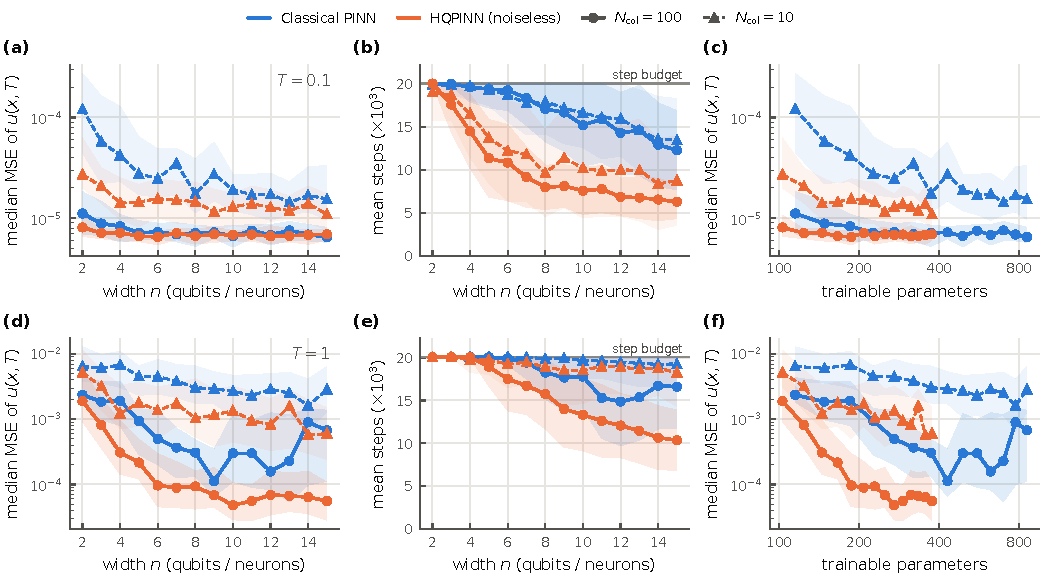
\includegraphics[width=\textwidth]{fig2_sim_width.pdf}
  \caption{\justifying Forward problem, more qubits or neurons: classical PINN (blue) and noiseless HQPINN (orange) with the same setup, for $T=0.1$ (top) and $T=1$ (bottom), with $\Ncol=100$ (circles, solid) and $\Ncol=10$ (triangles, dashed); 50 seeds per point.
  (a,d) Median MSE of $u(x,T)$ versus width $n$; bands, interquartile range.
  (b,e) Mean number of optimizer steps of the classical PINN divided by that of the HQPINN, over all runs, versus $n$ (logarithmic scale); above 1 the HQPINN needs fewer steps. Runs that miss the target count at the step budget.
  (c,f) Median MSE versus the number of trainable parameters.}
  \label{fig:width}
\end{figure*}

\paragraph{More qubits or neurons.} Figure~\ref{fig:width} shows the effect of the width $n$. At $T=0.1$ with $\Ncol=100$ both models reach the same error, a median MSE of $\simeq7\times10^{-6}$ ($\epsilon_{L_2}\simeq0.4\%$) for $n\ge5$, a level set by the reference solution [Fig.~\ref{fig:width}(a)]. What differs is the cost of getting there. The HQPINN uses about half of the optimizer steps, a factor between 1.95 and 2.16 for $n\ge7$, for example $7.6\times10^3$ against $1.52\times10^4$ at $n=10$ [Fig.~\ref{fig:width}(b)]. It also needs fewer parameters: an MSE of $8\times10^{-6}$ takes $n=3$ (124 parameters) against $n=5$ (226) [Fig.~\ref{fig:width}(c)]. And it is more reliable: for $n\ge5$, 98\% of its runs reach the target, against 55\% of the classical ones. With $\Ncol=10$ its median MSE is lower at every width, by a factor between 1.2 and 4.5, and an MSE of $3\times10^{-5}$ takes $n=2$ (103 parameters) against $n=5$ (226).

At $T=1$ the advantage extends to the error itself [Figs.~\ref{fig:width}(d)--(f)]. The median MSE of the HQPINN is lower at every width and for both values of $\Ncol$, by a factor of up to 14 for $\Ncol=100$; at $n=10$ it is $4.8\times10^{-5}$ ($\epsilon_{L_2}=3.3\%$) against $3.0\times10^{-4}$ (8.2\%), and 92\% of the runs reach the target against 34\%. An MSE of $10^{-4}$ takes $n=6$ (187 parameters), whereas the classical PINN does not reach it up to $n=15$ (856 parameters); its best median is $1.1\times10^{-4}$, at $n=9$. With $\Ncol=100$ the classical PINN uses between 1.16 and 1.6 times more steps for $n\ge7$. With $\Ncol=10$ neither model reaches the target in most runs (at most 20\% for the HQPINN and 12\% for the classical PINN), so both stay close to the budget and need about the same number of steps [Fig.~\ref{fig:width}(e)].

\begin{figure*}[t]
  \centering
  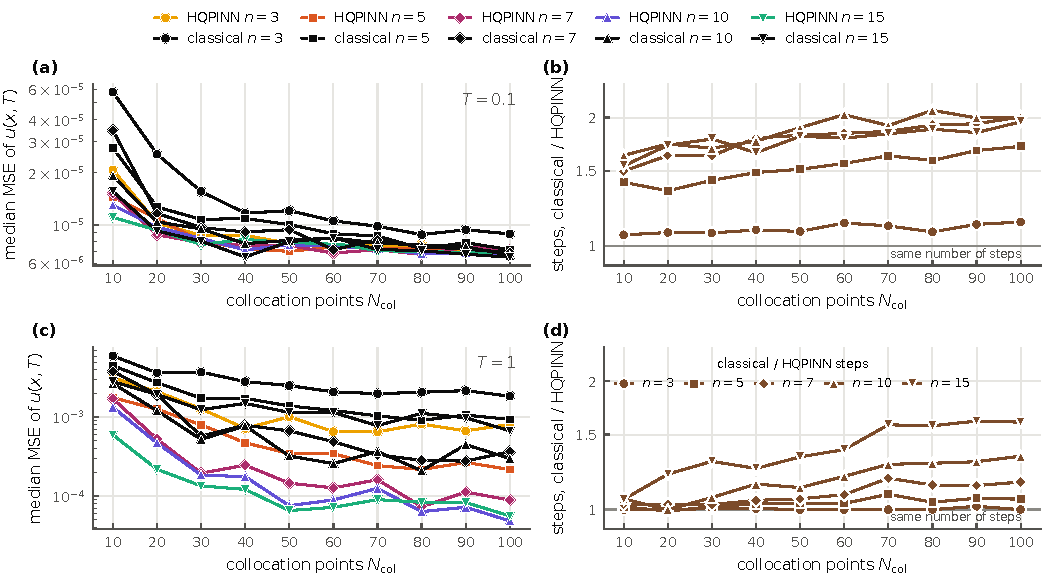
\includegraphics[width=\textwidth]{fig3_sim_points.pdf}
  \caption{\justifying Forward problem, more collocation points: noiseless HQPINN (colours, $\Ncol=10$ to 100) and classical PINN with the same setup (black, same range), with one marker per width $n=3,5,7,10,15$, at $T=0.1$ (top) and $T=1$ (bottom); 50 seeds per point. (a,c) Median MSE of $u(x,T)$. (b,d) Mean number of optimizer steps of the classical PINN divided by that of the HQPINN, over all runs, one curve per width, all in one colour and told apart by the marker (logarithmic scale); above 1 the HQPINN needs fewer steps. Runs that miss the target count at the step budget.}
  \label{fig:points}
\end{figure*}

\paragraph{More collocation points.} Figure~\ref{fig:points} shows the effect of $\Ncol$. At $T=0.1$ the median MSE of the HQPINN stays below $10^{-5}$ from $\Ncol=30$ on, for every width [Fig.~\ref{fig:points}(a)]. The number of steps depends much more on $n$ than on $\Ncol$: at $n=10$ it goes from $1.02\times10^4$ at $\Ncol=10$ to $7.6\times10^3$ at $\Ncol=100$. At $T=1$ the number of points matters more. For $n=10$, going from $\Ncol=10$ to 100 lowers the median MSE from $1.3\times10^{-3}$ to $4.8\times10^{-5}$, raises the fraction of runs that reach the target from 18\% to 92\% and lowers the mean number of steps from $1.85\times10^4$ to $1.33\times10^4$ [Fig.~\ref{fig:points}(c)]. The three-qubit model stays about an order of magnitude higher and at most 4\% of its runs reach the target, which identifies the width as the limiting factor at this horizon.

The classical curves compare the two models at every width and $\Ncol$. At $T=0.1$ the classical PINN uses more steps in all 50 configurations, by a factor of 1.1 to 1.7 for $n\le5$ and of 1.5 to 2.1 for $n\ge7$, and it reaches the target less often in all of them; at $n=10$, for example, in 52--64\% of its runs, against at least 94\% for the HQPINN from $\Ncol=20$ on [Fig.~\ref{fig:points}(b)]. The errors are close: from $\Ncol=20$ on and for $n\ge5$ the classical median is between 0.8 and 1.5 times that of the HQPINN. Only at $n=3$ is it clearly larger, by a factor of 1.1 to 2.8 [Fig.~\ref{fig:points}(a)].

At $T=1$ the median MSE of the classical PINN is larger in all 50 configurations, by a factor of 1.7 to 6.2 for $n\le10$ and of 4.7 to 18 for $n=15$ [Fig.~\ref{fig:points}(c)]. Among these five widths its best median is $2.1\times10^{-4}$ ($n=10$, $\Ncol=80$, 491 parameters); the HQPINN goes below that value with $n=7$ at $\Ncol=30$ (208 parameters). The saving in steps grows with $n$ and $\Ncol$ [Fig.~\ref{fig:points}(d)]. There is none at $n=3$, where at most 4\% of the runs of either model reach the target, and it reaches a factor of 1.33 at $n=10$ and 1.61 at $n=15$. The HQPINN reaches the target at least as often in 49 of the 50 configurations; the exception is $n=10$, $\Ncol=20$ (22\% against 24\%).

\subsection{Real quantum processor}\label{sec:f_qpu}
We trained the HQPINN with \texttt{ibm\_berlin} in the loop (Sec.~\ref{sec:hil}) for one specific case per horizon: $n=10$ qubits on 8 chains in parallel (80 of the 120 qubits), one job per epoch, 110 epochs, 1024 shots and no error mitigation (Appendix~\ref{app:fqpu}). This budget is two orders of magnitude below that of the simulations, so the runs do not reach the target; here we compare the error after the same number of epochs. Each result is a single run.

\begin{figure*}[t]
  \centering
  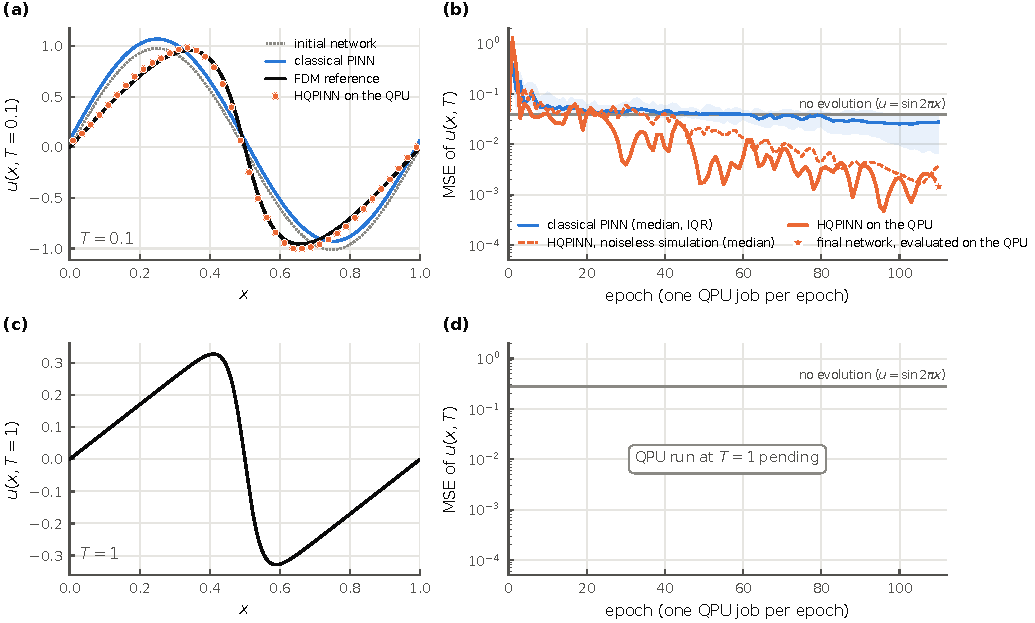
\includegraphics[width=\textwidth]{fig4_qpu.pdf}
  \caption{\justifying Forward problem, HQPINN trained with \texttt{ibm\_berlin} in the loop, one run per horizon. (a,b) $T=0.1$: $n=10$, $\Ncol=10$, 110 epochs, seed 0, no error mitigation. (a) $u(x,T)$: reference, initial network, classical PINN with the same protocol, seed and width, and HQPINN evaluated on the device (every fifth point). (b) MSE of $u(x,T)$ versus epoch, from the bit-exact replay of the recorded run, through the surrogate in force at each epoch; star, final network evaluated on the device. Blue, median and interquartile range of the classical PINN with the same protocol ($n=1,\dots,10$, seeds 0--4); dashed, median of the noiseless HQPINN (seeds 0--4). Grey, MSE of a network that does not evolve the initial condition. (c,d) $T=1$. \TODO{Pain\'eis (c,d) aguardam a rodada no QPU; (c) mostra s\'o a refer\^encia.}}
  \label{fig:qpu}
\end{figure*}

\paragraph{$T=0.1$.} The network starts at $\epsilon_{L_2}=29.4\%$ and ends at $\mathrm{MSE}=1.45\times10^{-3}$ ($\epsilon_{L_2}=5.7\%$) when evaluated with the circuit running on the device, a 27-fold reduction of the MSE, and it follows the steep front at $x\simeq0.5$ [Fig.~\ref{fig:qpu}(a)]. The classical PINN trained with the same protocol, seed and width has almost twice the parameters (491 against 271) and ends at 31.2\%, with the peak and the trough displaced. Over all 50 classical runs of the control ($n=1,\dots,10$, seeds 0--4) the median is 24.7\%, and only one run ends below the hardware MSE [Fig.~\ref{fig:qpu}(b)]. The classical schedule is the one selected for the HQPINN; the best of ten schedules tested for the classical PINN at $n=10$ gives 11.4\% (6.2--19.5\%), against 9.1\% (3.9--15.1\%) for the noiseless HQPINN with its own schedule. The hardware run lies within the spread of the noiseless model: after epoch 30 its learning curve is at or below the noiseless median in 88\% of the epochs, and the same weights evaluated with the ideal circuit give 6.0\%, so the network is not tied to the noise of the chip. Within the statistics of one run, device noise does not appear to be the limiting factor at this budget.

\paragraph{$T=1$.} \TODO{Resultado do QPU real em $T=1$.}

% =====================================================================
\section{Results: inverse problem}\label{sec:inverse}
% =====================================================================
Accuracy is measured by the relative error of the learned viscosity, $\epsilon_\nu=|\hat\nu-\nu_{\rm true}|/\nu_{\rm true}$, and by the relative error $\epsilon_{L_2}$ of $u(x,T)$ against the exact solution (Appendix~\ref{app:colehopf}).

\subsection{Simulation}\label{sec:i_sim}
Both models are trained with the same algorithm (Algorithm~\ref{alg:inv} in Appendix~\ref{app:isim}), with hyperparameters selected independently for each model under the same protocol. We use $\nu_{\rm true}=0.01$, $T\in\{0.1,1\}$, $\Ncol=10$ points per epoch, $n\in\{3,7,10\}$ and seeds 0--10, i.e., 33 runs per model and horizon. Runs with the same size and seed are paired: both models start from the same $\nu_0$ and see the same sequence of collocation points. At $T=1$ both models use the adjusted training of Appendix~\ref{app:adjust}. The quantum layer is evaluated on a noisy emulator of the device with $S=1024$ shots, in the loop of Sec.~\ref{sec:hil}: \texttt{FakeAachen} at the budget of $K=500$ epochs and \texttt{FakeBerlin} at $K=110$. The classical model runs without noise. Comparisons between the models use the two-sided paired Wilcoxon signed-rank test over the 33 pairs. Because the emulator changes together with the budget, the change of the HQPINN between 110 and 500 epochs mixes both effects; the classical model has no device, so its change is the effect of the epochs alone. Finally, the same 33 pairs per horizon were trained for $K=20\,000$ epochs with the noiseless layer (the ideal circuit), with the same algorithm, hyperparameters and adjustments; only the number of epochs changes, and the cosine decays stretch over it.


\begin{table}[t]
\caption{\justifying Inverse problem: relative error of the learned viscosity, $\epsilon_\nu$, and relative $L_2$ error of $u(x,T)$, over 33 paired runs per model ($\nu_{\rm true}=0.01$, $n\in\{3,7,10\}$, seeds 0--10). Wins: pairs in which the model has the smaller error; $p$: two-sided paired Wilcoxon test.}
\label{tab:inverse}
\setlength{\tabcolsep}{1pt}
\footnotesize
\begin{ruledtabular}
% written by manuscript/scripts/build_inverse_data.py: do not edit
\begin{tabular}{lcc}
 & HQPINN$^{b}$ & classical\\
\colrule
\multicolumn{3}{c}{$T=0.1$, $K=200$ (FakeAachen); $n=10$, 10 pairs}\\
\colrule
$\epsilon_\nu$ (\%)$^{a}$ & 1.9 / 3.7 / 11.6 & 4.6 / 6.5 / 18.0\\
$\epsilon_{L_2}$$^{a}$ & 0.011 / 0.013 / 0.018 & 0.009 / 0.011 / 0.016\\
wins ($\epsilon_\nu$; $\epsilon_{L_2}$) & 6; 4 & 4; 6\\
$p$ ($\epsilon_\nu$; $\epsilon_{L_2}$) & \multicolumn{2}{c}{0.43; 0.32}\\
\colrule
\multicolumn{3}{c}{$T=1$, $K=200$ (FakeAachen); $n=10$, 10 pairs}\\
\colrule
$\epsilon_\nu$ (\%)$^{a}$ & 36.9 / 32.1 / 71.4 & 18.0 / 24.9 / 52.2\\
$\epsilon_{L_2}$$^{a}$ & 0.063 / 0.068 / 0.099 & 0.050 / 0.052 / 0.067\\
wins ($\epsilon_\nu$; $\epsilon_{L_2}$) & 3; 3 & 7; 7\\
$p$ ($\epsilon_\nu$; $\epsilon_{L_2}$) & \multicolumn{2}{c}{0.23; 0.11}\\
\colrule
\multicolumn{3}{c}{$T=0.1$, $K=20\,000$ (noiseless); $n=3, 7, 10$, 33 pairs}\\
\colrule
$\epsilon_\nu$ (\%)$^{a}$ & 1.0 / 1.6 / 9.7 & 0.6 / 0.8 / 3.1\\
$\epsilon_{L_2}$$^{a}$ & 0.005 / 0.005 / 0.012 & 0.003 / 0.003 / 0.004\\
wins ($\epsilon_\nu$; $\epsilon_{L_2}$) & 11; 4 & 22; 29\\
$p$ ($\epsilon_\nu$; $\epsilon_{L_2}$) & \multicolumn{2}{c}{0.024; $2\times10^{-7}$}\\
\colrule
\multicolumn{3}{c}{$T=1$, $K=20\,000$ (noiseless); $n=3, 7, 10$, 33 pairs}\\
\colrule
$\epsilon_\nu$ (\%)$^{a}$ & 3.1 / 8.4 / 51.4 & 2.9 / 3.4 / 14.0\\
$\epsilon_{L_2}$$^{a}$ & 0.012 / 0.016 / 0.055 & 0.007 / 0.009 / 0.018\\
wins ($\epsilon_\nu$; $\epsilon_{L_2}$) & 12; 8 & 21; 25\\
$p$ ($\epsilon_\nu$; $\epsilon_{L_2}$) & \multicolumn{2}{c}{0.023; $1\times10^{-4}$}\\
\end{tabular}

\end{ruledtabular}
\raggedright\footnotesize $^{a}$Median / mean / max. $^{b}$At $K=110$ and 500, noisy emulator, with $u(x,T)$ evaluated with the circuit run on the emulator; at $K=20\,000$, ideal circuit.
\end{table}

\paragraph{Identification of the viscosity.} Table~\ref{tab:inverse} summarizes the results over all runs. At $T=0.1$ both models identify $\nu$ well and cannot be told apart: in 500 epochs the median $\epsilon_\nu$ is 2.8\% for the HQPINN and 2.3\% for the classical PINN ($p=0.76$; the HQPINN has the smaller error in 16 of the 33 pairs). The median error of both stays below 5\% from about epoch 400 on. The epochs help: from 110 to 500 the classical median goes from 7.3\% to 2.3\% (better in 28 of the 33 runs, $p<10^{-5}$), and that of the HQPINN from 6.0\% to 2.8\% (better in 24 of the 33 runs, $p=0.001$). At 110 epochs the models are also tied ($p=0.11$).

At $T=1$ the problem is harder for both models and more epochs do not solve it. The median $\epsilon_\nu$ goes from 21.5\% to 20.9\% for the classical PINN (better at 500 epochs in 13 of the 33 runs, $p=0.26$) and from 30.2\% to 30.5\% for the HQPINN (17 of 33, $p=0.82$), and the median of $\nu_k$ over the runs does not improve after about epoch 100. The classical PINN has the smaller median at both budgets, but the difference is significant only at 110 epochs ($p=0.046$, against $p=0.37$ at 500). Both models tend to underestimate $\nu$: at 500 epochs in 26 of the 33 classical runs and 30 of the 33 HQPINN runs, with final values down to $3.7\times10^{-3}$ and $2.5\times10^{-3}$. Across the sizes the medians vary widely and without a stable pattern: at 500 epochs, 41.2\%, 27.8\% and 12.8\% for the HQPINN with $n=3,7,10$, against 16.9\%, 33.7\% and 14.6\% for the classical PINN, whereas at 110 epochs $n=7$ is the best size of the HQPINN (Table~\ref{tab:persize}). With 11 seeds per size and a learned $\nu$ that still fluctuates by about 25\% over the last 20 epochs of a run (against 1.4--1.7\% at $T=0.1$), we do not interpret these differences. The final $\nu$ of a single run depends on the last batches, and comparisons require many seeds.

\paragraph{Long budget with the noiseless layer.} With $K=20\,000$ epochs both models identify $\nu$ at both horizons (Table~\ref{tab:inverse}). At $T=0.1$ the median $\epsilon_\nu$ is 1.0\% for the HQPINN and 0.6\% for the classical PINN, and at $T=1$ 3.1\% and 2.9\%; the classical PINN has the smaller error in 22 and 21 of the 33 pairs ($p=0.024$ and 0.023). At $T=1$ the epochs, not the device, make the difference for the classical model: its median goes from 20.9\% at 500 epochs to 2.9\%. The HQPINN with $n=3$ is the exception at this horizon, with a median of 11.7\% and a maximum of 51\%, which sets the mean of 8.4\%; with $n=7$ and 10 its median is 1.9\% and 2.2\%, against 2.9\% and 1.8\% for the classical PINN (Table~\ref{tab:persize}). The classical PINN again reconstructs the field better, with median $\epsilon_{L_2}=0.003$ against 0.005 at $T=0.1$ and 0.007 against 0.012 at $T=1$ (better in 29 and 25 of the 33 pairs). The learned $\nu$ still fluctuates at the end of the training: over the last 20 epochs its standard deviation is 0.4--0.8\% of $\nu$ at $T=0.1$ and 2--3\% at $T=1$ (medians over the runs).

Figure~\ref{fig:invtrain} shows the best run of each model at this budget, the one with the smallest $\epsilon_\nu$ among its 33 runs. At $T=0.1$ the best classical PINN ($n=3$, seed 9) learns $\hat\nu=0.01000$ ($\epsilon_\nu=0.03\%$) and the best HQPINN ($n=7$, seed 8) $0.00998$ (0.23\%); at $T=1$, $0.01000$ (0.04\%, $n=3$, seed 1) and $0.00999$ (0.06\%, $n=10$, seed 10). The corresponding $\epsilon_{L_2}$ are 0.003 and 0.005 at $T=0.1$ and 0.007 and 0.011 at $T=1$. In these runs $\nu_k$ reaches the neighbourhood of $\nu_{\rm true}$ within the first $10^2$ epochs and then fluctuates around it with a decreasing amplitude, while both terms of the loss keep decreasing until the end of the training. \TODO{Texto novo (20\,000 \'epocas, circuito ideal): revisar.}

\begin{figure*}[t]
  \centering
  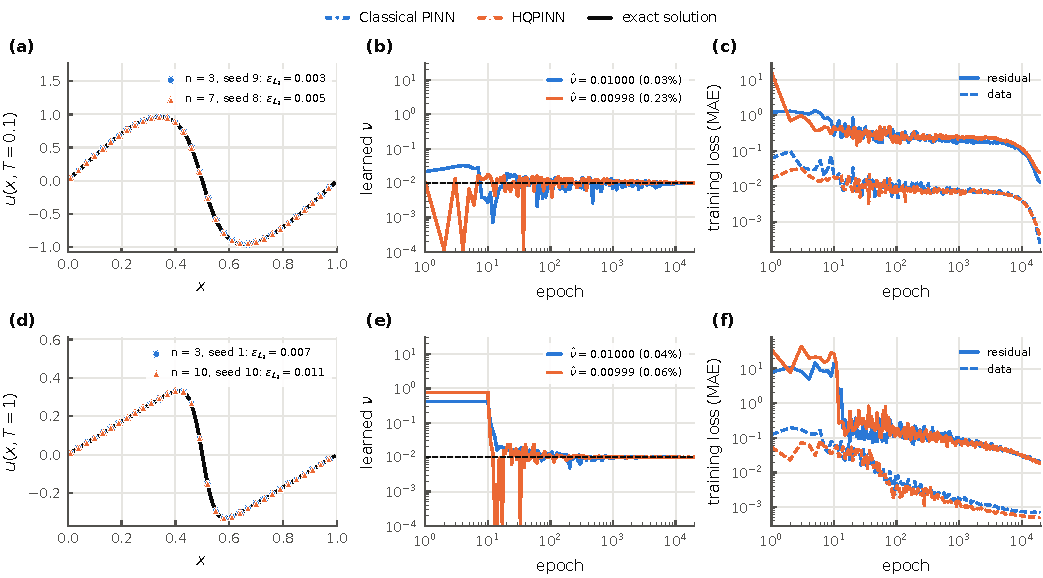
\includegraphics[width=\textwidth]{fig6_inv_training.pdf}
  \caption{\justifying Best run of each model at $K=20\,000$ epochs with the noiseless layer, the one with the smallest $\epsilon_\nu$ among its 33 runs (blue, classical PINN; orange, HQPINN with the ideal circuit), for $T=0.1$ (top) and $T=1$ (bottom). (a,d) $u(x,T)$ and the exact solution (every third point); the legend gives the size and seed of each run and $\epsilon_{L_2}$ of $u(x,T)$. (b,e) Learned viscosity versus epoch, with the final $\hat\nu$ and $\epsilon_\nu$ in the legend; dashed, $\nu_{\rm true}$; at $T=1$ the viscosity is frozen during the first 10 epochs. (c,f) The two terms of the training loss, the mean absolute error of the residual (solid) and of the data (dashed). In (b,c,e,f) the curves are medians over logarithmic bins of epochs (single epochs up to about epoch 25).}
  \label{fig:invtrain}
\end{figure*}

\paragraph{Reconstruction of the field.} The classical PINN, which runs without noise, reconstructs $u(x,T)$ better in all four cases (Table~\ref{tab:inverse}): at 500 epochs, median $\epsilon_{L_2}=0.005$ against 0.013 at $T=0.1$ (better in 32 of the 33 pairs) and 0.044 against 0.068 at $T=1$ (28 of 33). Unlike $\nu$, the field keeps improving with the epochs at $T=1$, from 0.073 to 0.044 for the classical PINN and from 0.107 to 0.068 for the HQPINN. A better field thus does not by itself give a better $\nu$ at this horizon. A likely cause is the small number of points per epoch: on a proxy of the device, more collocation points lowered the median $\epsilon_\nu$ of the HQPINN at $T=1$ markedly (Appendix~\ref{app:adjust}). \TODO{Com 20\,000 \'epocas e $\Ncol=10$ os dois modelos acertam $\nu$ em $T=1$: rever esta explica\c{c}\~ao.}

The networks of the HQPINN are trained through the noisy device, and they adapt to it. At $T=0.1$, the same weights combined with the ideal circuit give a larger error in 22 of the 33 runs at 500 epochs, by a median factor of 1.05 (25 of 33 and 1.14 at 110 epochs); at $T=1$ the effect disappears (17 of 33, median factor 1.00), the error being dominated by the front. This is the behaviour expected from Proposition~\ref{prop:trig}: noise changes the coefficients $c^{(q)}_{\bm\alpha}$ but not the function class, and the post-network learns the map from the coefficients of the device.

\subsection{Real quantum processor}\label{sec:i_qpu}
\TODO{Ainda n\~ao h\'a nenhuma rodada do problema inverso em hardware real: todos os resultados acima v\^em de emuladores. Esta se\c{c}\~ao e a Fig.~\ref{fig:invqpu} aguardam os dados. Sugest\~ao de texto a preencher: $\hat\nu$, $\epsilon_\nu$ e $\epsilon_{L_2}$ da rodada, comparados com a mediana e a dispers\~ao do emulador no mesmo or\c{c}amento.}
The training loop, the protocol and the comparison are ready. A run on a device uses the machinery of Sec.~\ref{sec:hil}, with the same training as on the emulator; at the budget of the forward run it costs 112 jobs (Appendix~\ref{app:iqpu}). Figure~\ref{fig:invqpu} holds the place of the result, which will be compared with the emulator medians at the same budget.

\begin{figure*}[t]
  \centering
  % 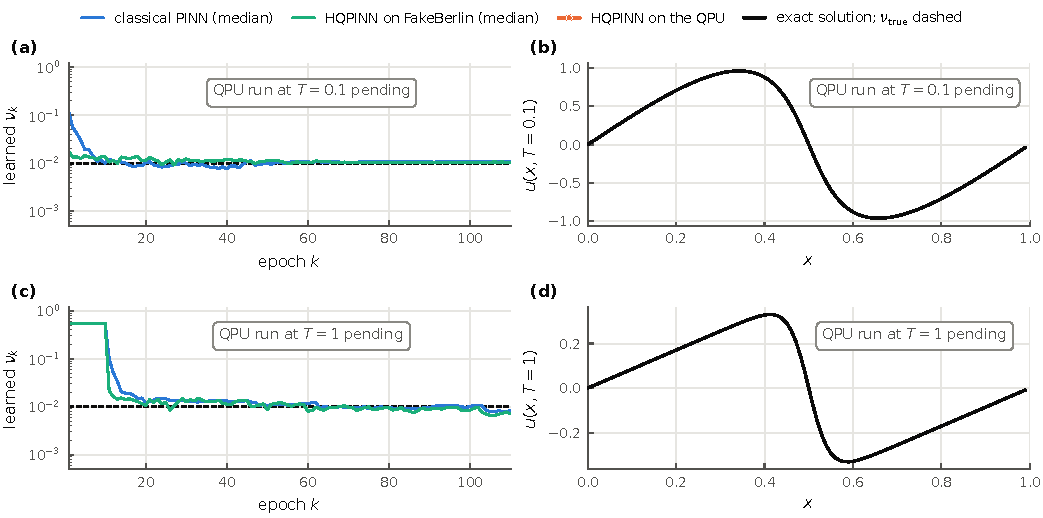
\includegraphics[width=\textwidth]{fig7_inv_qpu.pdf}
  \figspace{0.50\textwidth}
  \caption{\justifying Inverse problem on the real QPU. \TODO{A rodada ainda n\~ao existe; o script \texttt{fig7\_inv\_qpu.py} preenche os dados dela sozinho (\texttt{INVERSE\_QPU\_CASES} em \texttt{paper\_common.py}).} (a,c) Learned viscosity versus epoch at $K=110$: QPU run, and medians of the classical PINN and of the HQPINN on \texttt{FakeBerlin} over 33 runs; dashed, $\nu_{\rm true}$. (b,d) $u(x,T)$: QPU run and exact solution.}
  \label{fig:invqpu}
\end{figure*}

% =====================================================================
\section{Final considerations}\label{sec:discussion}
% =====================================================================
\TODO{Rascunho, a revisar depois das rodadas no QPU.}
In the forward problem, the simulations show that the HQPINN reaches the same error as the classical PINN with fewer parameters and fewer optimizer steps, and at the long horizon also a lower error. This comparison is between two classical computations: the noiseless quantum layer is a fixed cosine-product map, and its better conditioning of the residual minimization is an architectural effect. The quantum processor enters as the physical device that implements this map, and the hardware experiment addresses whether such a model can be \emph{trained} through a noisy device. At the budget tested the answer is positive: with one job per epoch, without error mitigation, on 80 qubits, the network reaches an accuracy within the spread of the noiseless model trained with the same protocol. This is possible because noise changes the coefficients of the layer but not its functional form, so a calibrated model of the device provides both the gradient and a noise-free interpolation across the finite-difference stencil.

In the inverse problem we find no advantage of the HQPINN at the budgets and with the noise tested. In the short runs on the emulator the two models identify $\nu$ equally well at $T=0.1$, neither identifies it accurately at $T=1$, and the classical PINN reconstructs the field better throughout. The same training machinery works in both problems, but the two sets of results should not be read as one comparison. The forward simulations are noiseless, long and stop at a physical target; the inverse runs are short, fixed-budget, and put the noise of the device on the HQPINN only. In addition, the hyperparameters of the inverse runs were selected at $\nu=0.1$, $T=0.1$ and not at the values used here. The direct counterpart of Sec.~\ref{sec:f_sim} for the inverse problem, a noiseless HQPINN and a classical PINN under one protocol, is the long-budget run of Sec.~\ref{sec:i_sim}: with $20\,000$ epochs both models identify $\nu$ at both horizons, with a slightly smaller error for the classical PINN (Appendix~\ref{app:long}). For the classical PINN, which is noiseless in the short runs too, the failure at $T=1$ at 110 and 500 epochs is therefore a matter of budget; for the HQPINN the comparison mixes the budget with the noise of the emulator. \TODO{Rodar o controle cl\'assico com produto de cossenos [Eq.~\eqref{eq:parity}] separaria o efeito da arquitetura do efeito do ru\'ido.}

\emph{Limitations.} The hardware results rest on a single run per horizon, the seed at $T=0.1$ was the best of five on an emulator of the device, and the real-QPU results at $T=1$ (forward) and for the inverse problem are still missing. The classical family compared here has one specific middle block, and in the forward problem the common protocol does not use separately optimized hyperparameters for each model; at the hardware budget a schedule tuned for the classical PINN narrows the gap to the noiseless HQPINN (Appendix~\ref{app:controls}). The target and the error metric of the forward problem rely on a first-order finite-difference reference whose own error sets the $7\times10^{-6}$ floor at $T=0.1$. The emulators reproduce the calibrated errors of the device but not crosstalk or drift, and they do not fix the seed of the simulator, so rerunning the HQPINN gives slightly different numbers. In the inverse problem, the effects of the budget and of the emulator on the HQPINN were not separated.

% =====================================================================
\section{Conclusions}\label{sec:conclusions}
% =====================================================================
\TODO{Rascunho -- revisar; incluir $T=1$ no QPU e o problema inverso em hardware real, e o problema inverso com 20\,000 \'epocas (circuito ideal).} A PINN with a fixed, parameter-free quantum layer needs fewer trainable parameters and fewer optimizer steps than a classical PINN of the same form to reach the same error on the viscous Burgers equation: about half of the steps at $T=0.1$ and, at $T=1$ and $n=10$, an error about 6 times lower. Since the noiseless layer is classically computable, this is a property of the architecture. The model can also be trained with a superconducting quantum processor in the loop, with one job per epoch and no error mitigation: at $T=0.1$ it reaches $\epsilon_{L_2}=5.7\%$ in 110 epochs, in line with the noiseless simulation at the same budget. The same model and loop extend to the inverse problem, with the viscosity updated in closed form. With the layer on a noisy emulator it identifies the viscosity as well as the classical PINN at $T=0.1$ (median error 2.8\% against 2.3\% in 500 epochs), and it does not improve on it at $T=1$, where neither model is accurate.

\section*{Data and code availability}\label{sec:data}
\TODO{Reposit\'orio/Zenodo.} The tables behind every figure are in \texttt{manuscript/data/}, written from the raw results in \texttt{data/} by \texttt{manuscript/scripts/build\_paper\_data.py}; \texttt{manuscript/scripts/make\_all.py} regenerates tables and figures. \texttt{replay\_training.py}, \texttt{simulate\_same\_budget.py} and \texttt{controls\_hardware\_budget.py} produce the replayed learning curves and the hardware-budget controls without any quantum job. The IBM job identifiers of all 113 hardware jobs are recorded in the run logs.

\begin{acknowledgments}
\TODO{Agradecimentos; acesso ao IBM Quantum (inst\^ancia PDE\_Europe); financiamento.}
\end{acknowledgments}

% =====================================================================
\begin{appendices}
% =====================================================================

% ---------------------------------------------------------------------
\section{Forward problem: simulation}\label{app:fsim}
% ---------------------------------------------------------------------
\renewcommand{\thesubsection}{\thesection.\arabic{subsection}}
\makeatletter\renewcommand{\p@subsection}{}\makeatother

\subsection{Reference solution and error metrics}\label{app:reference}
The reference $u_{\rm FDM}$ is obtained with an explicit scheme on $N_x=512$ periodic grid points ($\Delta x=1/512$) with time step $\Delta t=10^{-4}$: first-order upwind differences for the advection term, $u\,\partial_xu\to u_j(u_j-u_{j-1})/\Delta x$ for $u_j\ge0$ and $u_j(u_{j+1}-u_j)/\Delta x$ otherwise, and second-order central differences for the diffusion term. The time step satisfies the advective and diffusive stability limits ($\Delta t\max|u|/\Delta x\simeq0.05$, $\nu\Delta t/\Delta x^2\simeq0.26$). Evaluation points that do not coincide with the grid are obtained by periodic linear interpolation at $t=T$. The reference is used only for evaluation: $\nu$ is known and there is no solution data in the training.

\emph{FDM floor.} The stopping target of the simulations is the residual of the reference itself, $\mathcal L_{\rm FDM}=\frac{1}{N}\sum_k r_k[u_{\rm FDM}]^2$, evaluated with the same stencil $(h,\tau)$ on the same validation points, with $u_{\rm FDM}$ interpolated bilinearly (periodic in $x$, linear in $t$). Because the upwind scheme is only first-order accurate, $\mathcal L_{\rm FDM}>0$; a network whose residual is below it would be fitting the error of the reference. The corresponding floor of the MSE against the reference is $\simeq7\times10^{-6}$ at $T=0.1$. It is the error of the reference itself: against the exact solution of Appendix~\ref{app:colehopf}, on 2000 points, $u_{\rm FDM}$ has an MSE of $6.9\times10^{-6}$ at $T=0.1$ and $4.0\times10^{-6}$ at $T=1$.

\emph{Metrics.} $\mathrm{MSE}=\frac1P\sum_p[u(x_p,T)-u_{\rm FDM}(x_p,T)]^2$, $\mathrm{MAE}$ analogously, and $\epsilon_{L_2}=\|u-u_{\rm FDM}\|_2/\|u_{\rm FDM}\|_2$, on $P=200$ equispaced points $x_p\in[0,1]$. At $T=0.1$, $\langle u_{\rm FDM}^2\rangle=0.453$, so $\epsilon_{L_2}=\sqrt{\mathrm{MSE}/0.453}$. A model that does not evolve the initial condition, $u(x,T)=\sin2\pi x$, has $\mathrm{MSE}=3.93\times10^{-2}$ at $T=0.1$ and $2.82\times10^{-1}$ at $T=1$.

\subsection{Architectures and hyperparameters}\label{app:hyper}

\begin{table}[h]
\caption{\justifying Network architectures (all hidden layers $\tanh$, linear outputs), for the two problems. The forward simulations use $m=n$; the classical control at the hardware budget and the inverse problem use $m=10$. The two coincide at $n=10$. The learnable $\nu$ is not counted.}
\label{tab:arch}
\setlength{\tabcolsep}{2pt}
\footnotesize
\begin{ruledtabular}
\begin{tabular}{lcc}
 & HQPINN & classical PINN\\
\colrule
features & $\bm\xi$, Eq.~\eqref{eq:composition} & same\\
$\mathcal N_{\rm pre}$ & $3\to10\to n$ & $3\to10\to n$\\
middle block & $R_Y$, $W_{\rm brick}$, $\langle Z_q\rangle$ & $n\to m\to n$\\
$\mathcal N_{\rm post}$ & $n\to10\to1$ & $n\to10\to1$\\
param., middle & 0 & $2nm+m+n$\\
param., total & $21n+61$ & $2n^2+23n+61$ $(m{=}n)$\\
 & & $42n+71$ $(m{=}10)$\\
$n=3,7,10$ & 124, 208, 271 & 197, 365, 491 $(m{=}10)$\\
\end{tabular}
\end{ruledtabular}
\end{table}

\begin{table}[h]
\caption{\justifying Training hyperparameters of the forward simulations (Figs.~\ref{fig:width} and~\ref{fig:points}), identical for both models.}
\label{tab:hyper_sim}
\setlength{\tabcolsep}{2pt}
\footnotesize
\begin{ruledtabular}
\begin{tabular}{lc}
$\Ncol$ per step & 10--100\\
stencil $(h,\tau)$ & $(1/512,10^{-3})$\\
optimizer & AdamW, L-BFGS\\
steps & $\le2{\times}10^4+10^3$\\
learning rate & $10^{-3}$, plateau $\times\frac12$\\
weight decay; gradient clip & $10^{-6}$; 1\\
L-BFGS & lr 0.5, history 50\\
stopping & FDM floor\\
seeds & 0--49\\
\end{tabular}
\end{ruledtabular}
\end{table}

\subsection{Simulation protocol}\label{app:sim}
Both models are trained with the same algorithm and hyperparameters (Algorithm~\ref{alg:sim}): AdamW~\cite{loshchilov2019decoupled} with learning rate $10^{-3}$ reduced on plateaus, a fresh batch of $\Ncol$ collocation points at every step, up to $2\times10^4$ steps, followed by at most $10^3$ L-BFGS iterations~\cite{liu1989limited} on the last batch. The residual is monitored on a fixed validation set of $\Ncol$ random points, and training stops when it reaches the FDM floor on the same points and with the same stencil (Appendix~\ref{app:reference}). The best monitored snapshot is returned. We sweep $n=2,\dots,15$, $\Ncol\in\{10,100\}$ and $T\in\{0.1,1\}$, with 50 seeds per configuration and model (5600 runs), seed $s$ fixing the initialization and the validation set. Complementary sweeps under the same protocol cover $\Ncol$ from 10 to 100, for both models at $n\in\{3,5,7,10,15\}$. \TODO{arquivar no reposit\'orio o script que gerou a varredura (\texttt{Experiment1Modified}, protocolo \texttt{fixed\_validation\_v2}); \texttt{run\_qubit\_sweep.py --fixed-validation} reproduz o protocolo, conferido em 14 seeds.} The ideal quantum layer is evaluated with the closed form~\eqref{eq:parity}, which is exact for the noiseless circuit and differentiable. Neither model has failed runs at $T=0.1$ (largest MSE $2.2\times10^{-3}$ for the classical PINN and $1.2\times10^{-3}$ for the HQPINN among 1400 runs each).

\begin{algorithm}{Forward simulation training (classical PINN and ideal HQPINN), long budget.}\label{alg:sim}
\item \textbf{input:} width $n$, $\Ncol$, horizon $T$, seed $s$; stencil $(h,\tau)$; $K_{\rm A}=2\times10^4$, $K_{\rm B}=10^3$
\item set seed $s$; initialize $\Theta$; draw a fixed validation set $\mathcal V$ of $\Ncol$ points (seed $10^6+s$)
\item $\mathcal L_{\rm FDM}\gets$ residual of the reference on $\mathcal V$ (Appendix~\ref{app:reference})
\item \textbf{for} $k=1,\dots,K_{\rm A}$: draw $\Ncol$ points; build the $5\Ncol$ stencil nodes; $\Theta\gets$ AdamW$(\nabla_\Theta\mathcal L)$; evaluate $\mathcal L(\mathcal V)$; keep the best snapshot; \textbf{stop} if $\mathcal L(\mathcal V)\le\mathcal L_{\rm FDM}$
\item restore the best snapshot; \textbf{for} $k=1,\dots,K_{\rm B}$: one L-BFGS iteration on the last batch; evaluate $\mathcal L(\mathcal V)$; \textbf{stop} at the target or after 50 iterations without improvement
\item \textbf{return} the best snapshot
\end{algorithm}

\subsection{The noiseless quantum layer}\label{app:parity}
The first sublayer of $W_{\rm brick}$ acts on the pairs $(1,2),(3,4),\dots$ and the second on $(2,3),(4,5),\dots$ ($n-1$ gates in total).
\begin{remark}\label{rem:parity}
    A CNOT network acts on the computational basis as a linear map over $\mathrm{GF}(2)$, $\bm b\mapsto M\bm b$. For the noiseless circuit~\eqref{eq:circuit} the Heisenberg evolution of $Z_q$ is the Pauli string $\prod_{j\in\mathcal S_q}Z_j$ with $\mathcal S_q=\{j:M_{qj}=1\}\subseteq\mathcal C_q$, and
    \begin{equation}
      y_q(\bm\theta)=\prod_{j\in\mathcal S_q}\cos\theta_j ,\qquad |\mathcal S_q|\le3 .
      \label{eq:parity}
    \end{equation}
    The ideal layer is therefore efficiently classically computable: the noiseless HQPINN is a classical network with cosine-product activations. Its simulation results measure the merit of this \emph{architecture}, not a quantum advantage, in line with the general results on classical surrogates of quantum learning models~\cite{schreiber2023classical}. For angles spread over a full period, $\operatorname{Var}[y_q]=2^{-|\mathcal S_q|}$, so deeper entangling layers trade expressivity (longer products) against concentration.
\end{remark}

\emph{Proof.} CNOT conjugation maps $Z_c\mapsto Z_c$ and $Z_t\mapsto Z_cZ_t$, so $Z_q$ evolves into the string $Z_{\mathcal S_q}$ whose support is the $q$th row of the GF(2) matrix $M$ of the network. On $\bigotimes_jR_Y(\theta_j)|0\rangle$, $\langle Z_j\rangle=\cos\theta_j$ and the state is a product, which gives Eq.~\eqref{eq:parity}. For one brickwork layer on $n=10$ qubits the supports are $\mathcal S_1=\{1\}$, $\mathcal S_2=\{1,2\}$, $\mathcal S_{q}=\{q-2,q-1,q\}$ for odd $q\ge3$, $\mathcal S_q=\{q-1,q\}$ for even $q\ge4$, so that, e.g., $y_3=\cos\theta_1\cos\theta_2\cos\theta_3$ and $y_{10}=\cos\theta_9\cos\theta_{10}$; hence $|\mathcal S_q|\le3$ and $\mathcal S_q\subsetneq\mathcal C_q$ for most outputs. If the $\theta_j$ are independent and uniform on a period, $\mathbb E[\cos^2\theta_j]=1/2$, hence $\operatorname{Var}[y_q]=2^{-|\mathcal S_q|}$ and $\mathbb E[(\partial_{\theta_j}y_q)^2]=2^{-|\mathcal S_q|}$.

% ---------------------------------------------------------------------
\section{Forward problem: real hardware}\label{app:fqpu}
% ---------------------------------------------------------------------

\subsection{Proof of Proposition~\ref{prop:trig}}\label{app:trig}
On hardware, $\hat y_q=y_q+\xi_q$ with $\mathbb E[\xi_q]=0$ and $\operatorname{Var}[\xi_q]=(1-y_q^2)/S\le1/S$. The hypothesis of Proposition~\ref{prop:trig} holds on IBM devices because $R_Y(\theta)$ is compiled into fixed microwave pulses and a \emph{virtual} $R_Z$ rotation, so the physical operations, and hence their errors, do not depend on $\theta$. Equation~\eqref{eq:trigpoly} has three consequences. (i) The quantum layer injects a finite Fourier structure into the latent representation~\cite{schuld2021effect}: the pre-network learns where to place the angles, and the circuit multiplies harmonics of different latent coordinates, $\cos\theta_a\cos\theta_b=\tfrac12[\cos(\theta_a+\theta_b)+\cos(\theta_a-\theta_b)]$, in the spirit of Fourier-feature networks~\cite{tancik2020fourier,rahimi2007random}. (ii) Noise does not change the function class, only the coefficients; this is what makes a calibrated surrogate of the device possible. (iii) The quantum layer has no trainable parameter, so what remains of the barren-plateau question is the possible concentration of the map $\bm\theta\mapsto\bm y$ itself, which is controlled by the size of the light cones (Remark~\ref{rem:parity}). The fixed layer connects the HQPINN to fixed-substrate approaches such as quantum feature maps~\cite{havlicek2019supervised}, quantum reservoir computing and extreme learning machines~\cite{fujii2017harnessing,mujal2021opportunities} and quanvolutional networks~\cite{henderson2020quanvolutional}, none of which has been used to minimize a PDE residual.

\emph{Trigonometric structure.} For a single rotation,
\begin{align}
  R_Y(\theta)\,\rho\,R_Y^\dagger(\theta)={}&\tfrac12(\rho+Y\rho Y)+\tfrac12\cos\theta\,(\rho-Y\rho Y)\nonumber\\
  &-\tfrac{i}{2}\sin\theta\,[Y,\rho],
  \label{eq:ry_channel}
\end{align}
so the map $\rho\mapsto R_Y(\theta)\rho R_Y^\dagger(\theta)$ is an affine combination of $\{1,\cos\theta,\sin\theta\}$ with $\theta$-independent superoperators. All other operations---CNOTs, noise channels, readout confusion matrices and the trace with $Z_q$---are linear and $\theta$-independent. Since each angle appears in exactly one gate, $y_q$ is a sum of products in which every $\theta_j$ contributes exactly one factor in $\{1,\cos\theta_j,\sin\theta_j\}$, which is Eq.~\eqref{eq:trigpoly}.

\emph{Light cone.} In the Heisenberg picture $y_q=\operatorname{Tr}[\rho_0\,\mathcal E^\dagger_{\bm\theta}(Z_q)]$. The adjoint of a trace-preserving channel is unital, so every gate (and every gate-local noise channel) whose support does not intersect the current support of the evolved operator leaves it unchanged. The support grows only through gates that touch it; the set of qubits reached is $\mathcal C_q$, and rotations outside $\mathcal C_q$ drop out. Going backwards through one brickwork layer, the second sublayer adds at most the partner of $q$ and the first sublayer at most one qubit on each side, so $|\mathcal C_q|\le4$; for $D$ layers, $|\mathcal C_q|\le\min(n,4D)$. For $n=10$ the cones are $\{1,2\}$, $\{1,\dots,4\}$ (twice), $\{3,\dots,6\}$ (twice), $\{5,\dots,8\}$ (twice), $\{7,\dots,10\}$ (twice) and $\{9,10\}$. Crosstalk or non-local noise invalidates this bound and enlarges the effective cone.

\emph{Conditioning of the calibration.} With $\theta_j\sim\mathcal U(-\pi,\pi)$ i.i.d., the features $\prod_{j\in\mathcal C_q}g_{\alpha_j}(\theta_j)$ are orthogonal, with $\mathbb E[g_0^2]=1$ and $\mathbb E[g_c^2]=\mathbb E[g_s^2]=1/2$. The Gram matrix of the least-squares problem is therefore diagonal in expectation, with condition number $2^{|\mathcal C_q|}\le16$, and the standard error of a coefficient with $k$ non-constant factors is $\simeq\sigma\,2^{k/2}/\sqrt{N_{\rm cal}}$. With $N_{\rm cal}=1024$ samples and $\sigma\simeq1/32$, the highest-order coefficients ($k=4$) are determined to $\simeq4\times10^{-3}$, well below the shot noise of a single measurement.

\subsection{The loop on a device}\label{app:hil}
\paragraph{Why a surrogate.} The device returns $\hat{\bm y}$ but not $\partial\bm y/\partial\bm\theta$. Parameter-shift rules~\cite{mitarai2018quantum,schuld2019evaluating,wierichs2022general} give unbiased derivatives at the price of $2n$ extra circuits per evaluation point, and SPSA~\cite{spall1992multivariate,kandala2017hardware} gives a single random directional derivative per step. If the five stencil nodes were measured independently, the shot noise $\sigma_u$ of $u$ would also enter $\partial_x^2u$ amplified by $\sqrt6/h^2\approx6.4\times10^5$ (Appendix~\ref{app:ste}).

\paragraph{The three stages.} \emph{Calibration:} before training, one job evaluates the circuit at random angles $\theta_j\sim\mathcal U(-\pi,\pi)$ on every $n$-qubit chain of the chip in parallel; the coefficients of Eq.~\eqref{eq:trigpoly} are obtained by linear least squares, which yields a surrogate $\hat f(\bm\theta)$ of the device with its average noise built in~\cite{sung2020using}. \emph{Training:} Eq.~\eqref{eq:ste} at each epoch. At the centre $\tilde{\bm y}=\hat{\bm y}^{\,\rm QPU}$, so the value of $u$ entering the nonlinear term $u\,\partial_xu$ is the measured one; across the stencil the variation of $\tilde{\bm y}$ is that of the smooth surrogate; and the gradient is $\partial\tilde{\bm y}/\partial\bm\theta=\partial\hat f/\partial\bm\theta$, available analytically. Every $K_{\rm fit}$ epochs the surrogate is refitted with the calibration data and all measurements accumulated so far, so that it tracks the device in the region of angles actually visited by the network. \emph{Validation:} a final job evaluates $u(x,T)$ with the trained network and the circuit run on the device. Because the surrogate has the exact functional form of the device response, the method does not approximate the circuit; its only bias is the statistical error of the fitted coefficients and the part of the device behaviour that the time-independent, chip-averaged model~\eqref{eq:trigpoly} cannot capture (chain-to-chain variation, drift, crosstalk). The construction applies to any circuit whose light cones are small enough for the $3^{|\mathcal C_q|}$ coefficients of Eq.~\eqref{eq:trigpoly} to be calibrated, which bounds the entangling depth to a few brickwork layers, and it is compatible with error mitigation schemes that are affine in the measured data (e.g., readout mitigation~\cite{vandenberg2022model}, Pauli twirling, linear zero-noise extrapolation~\cite{temme2017error}).

\begin{algorithm}{Forward HQPINN training with the quantum processor in the loop.}\label{alg:hil}
\item \textbf{input:} chains $\{\mathcal Q_b\}_{b=1}^{B}$, shots $S$, epochs $K$, $\Ncol$, refit period $K_{\rm fit}$, schedule $\eta_k$
\item \emph{calibration job}: $\lceil1024/B\rceil$ random angle sets on all chains $\to(\bm\theta,\hat{\bm y})$; screen chains; fit $\hat f$ [Eq.~\eqref{eq:trigpoly}]
\item set seed; initialize $\Theta=(\bm\phi,\bm\psi)$
\item \textbf{for} $k=1,\dots,K$:
\item \quad draw $\Ncol$ centres; stencil nodes $\mathcal S$; $\bm\theta\gets\mathcal N_{\rm pre}(\bm\xi(\mathcal S))$
\item \quad \emph{job $k$}: measure $\hat{\bm y}_c$ at the centres; centre $p$ runs on chain $(p+k)\bmod B$
\item \quad $\tilde{\bm y}\gets\hat f(\bm\theta)+\sg[\hat{\bm y}_c-\hat f(\bm\theta_c)]$ on all nodes [Eq.~\eqref{eq:ste}]
\item \quad $u\gets$ Eq.~\eqref{eq:composition}; $\mathcal L\gets$ Eq.~\eqref{eq:loss}; backward through $\hat f$; clip $\|\nabla\|\le1$; AdamW step with $\eta_k$
\item \quad \textbf{if} $k\bmod K_{\rm fit}=0$: refit $\hat f$ with the calibration and all measurements so far
\item \emph{validation job}: $u(x,T)$ on 200 points, each measured on every chain and averaged
\end{algorithm}

The learning rate is set at every epoch, $\eta_k=\max\{0.1-0.01\lfloor(k-1)/10\rfloor,\,0.01\}$, and the AdamW state is kept across epochs.

\begin{table}[h]
\caption{\justifying Hyperparameters at the hardware budget: \texttt{ibm\_berlin}, FakeBerlin, classical control and hardware-budget simulations (Fig.~\ref{fig:qpu}, Appendix~\ref{app:controls}).}
\label{tab:hyper_hw}
\setlength{\tabcolsep}{2pt}
\footnotesize
\begin{ruledtabular}
\begin{tabular}{lc}
$\Ncol$ per epoch & 10\\
stencil $(h,\tau)$ & $(1/512,10^{-3})$\\
optimizer; steps & AdamW; 110\\
learning rate & 0.1 to 0.01\\
weight decay; gradient clip & $10^{-6}$; 1\\
stopping & fixed budget\\
shots $S$ & 1024\\
calibration & 1024 samples\\
refit $K_{\rm fit}$ & 10 epochs\\
seeds & 0 (QPU), 0--4\\
\end{tabular}
\end{ruledtabular}
\end{table}

\subsection{The run at \texorpdfstring{$T=0.1$}{T=0.1}}\label{app:run}
The hardware experiment ran on \texttt{ibm\_berlin}, an IBM Nighthawk processor with 120 transmon qubits on a square lattice and native CZ gates, on 8 October 2026, within a single dedicated runtime \texttt{Session}. The circuit~\eqref{eq:circuit} with $n=10$ was laid out on 8 disjoint chains of 10 coupled qubits (Fig.~\ref{fig:chip}), selected from the current calibration data (12 candidate chains, 4 discarded for a high error score), and the 8 copies were transpiled into a single packed circuit of depth 12 with 72 CZ gates and no SWAPs. All expectation values were estimated with $S=1024$ shots (precision $1/32$) and \emph{without} error suppression or mitigation (raw counts). The run consisted of one calibration job (128 parameter sets on 8 chains, 1024 samples per output), 110 training jobs (one per epoch, the 10 stencil centres distributed over the chains) and one validation job (200 points, each measured once on every chain and averaged), i.e., 112 jobs, 548 parameter sets and $5.6\times10^5$ shots in 54~min of wall-clock time. Training used AdamW with learning rate $0.1$ decreased by $0.01$ every 10 epochs down to $0.01$, gradient-norm clipping at 1 and $K_{\rm fit}=10$. The hardware seed (seed 0) is the best of an earlier FakeBerlin batch of five seeds. Device characteristics are listed in Table~\ref{tab:device}.

\begin{figure}[t]
  \centering
  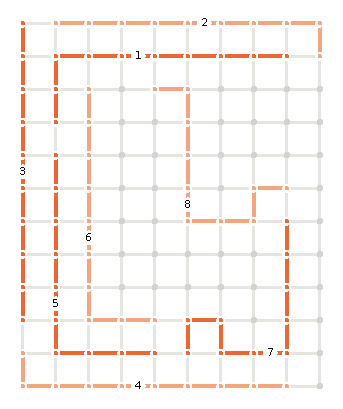
\includegraphics[width=0.72\linewidth]{figB1_chip.pdf}
  \caption{\justifying The 120-qubit square lattice of \texttt{ibm\_berlin} and the 8 disjoint 10-qubit chains on which the circuit ran in parallel (alternating shades and numbers distinguish neighbouring chains).}
  \label{fig:chip}
\end{figure}

\begin{table}[b]
\caption{\justifying \texttt{ibm\_berlin} on 8 October 2026: the 80 qubits and 72 couplers used (median and range).}
\label{tab:device}
\setlength{\tabcolsep}{4pt}
\footnotesize
\begin{ruledtabular}
\begin{tabular}{lcc}
quantity & median & range\\
\colrule
$T_1$ & 322~$\mu$s & 110--528~$\mu$s\\
$T_2$ & 255~$\mu$s & 34--510~$\mu$s\\
readout error & 1.7\% & 0.5--6.3\%\\
$\sqrt X$ error & $1.7\times10^{-4}$ & $(0.7$--$9.9)\times10^{-4}$\\
CZ error & $1.7\times10^{-3}$ & $(0.6$--$14)\times10^{-3}$\\
\colrule
qubits used / total & \multicolumn{2}{c}{80 / 120 (8 chains $\times$ 10)}\\
packed circuit & \multicolumn{2}{c}{depth 12, 72 CZ, no SWAP}\\
jobs / shots / time & \multicolumn{2}{c}{112 / $5.6\times10^5$ / 54 min}\\
\end{tabular}
\end{ruledtabular}
\end{table}

\paragraph{Chains.} All disjoint chains of $n$ physically coupled qubits are searched on the coupling map with a randomized greedy depth-first search that starts from the qubits with fewest free neighbours (100 trials; the largest set is kept). Each chain is scored by the sum of its readout and $\sqrt X$ errors and of the CZ errors of its links, and chains with a score above $0.05\,n$ are discarded; on \texttt{ibm\_berlin} 8 of 12 candidate chains were kept (rejected scores 0.51, 0.57, 1.27, 3.83). The circuit is laid out on all kept chains in a single packed circuit, so that one parameter set yields one sample per chain; transpilation with an initial layout on the chains produced no SWAP (72 CZ, depth 12).

\paragraph{Calibration and screening.} The calibration job evaluates 128 random angle sets on the 8 chains (1024 samples per output). Since the chains are physically different, each chain is also screened: its RMS misfit to the chip-averaged surrogate is computed, and chains above three times the median are discarded. On \texttt{ibm\_berlin} the misfits were 0.032--0.080 and all chains were kept. The surrogate is a single set of coefficients for the whole chip; the per-output fit RMS was 0.025--0.095 (mean 0.039, shot noise 0.031) and the RMS difference between the device and the ideal formula 0.064 (FakeBerlin: 0.028 and 0.039).

\paragraph{Training jobs.} The 10 stencil centres of each epoch fill 2 parameter sets on the 8 chains; centre $p$ runs on chain $(p+k)\bmod8$ at epoch $k$, which rotates the points over the chains and prevents a systematic assignment of points to poor chains. The surrogate is refitted every 10 epochs with the calibration data and all training measurements (1124 to 2124 samples). An epoch took 16~s on average, dominated by job latency inside the session; on the emulator, 3.5~s.

\paragraph{Validation.} The validation job evaluates the 200 points at $t=T$ with 8 replicas, one on every chain, and averages $\hat{\bm y}$ over the replicas before the post-network, so the average matches the chip-averaged surrogate. Three evaluations of the same weights give $\epsilon_{L_2}=5.7\%$ with the circuit on the device, 5.5\% with the surrogate and 6.0\% with the ideal formula.

\paragraph{Offline replay.} The run log contains the initial weights, the calibration data and, for every epoch, the collocation points, the angles sent to the device and the measured $\hat{\bm y}$. Replaying Algorithm~\ref{alg:hil} with the recorded measurements in place of the device reproduces the trained weights, the training losses and the angles of every epoch exactly (maximum difference zero, for both \texttt{ibm\_berlin} and FakeBerlin), which we use to evaluate the network after each epoch [Fig.~\ref{fig:qpu}(b)] without additional quantum resources. This holds on the software stack of the run (Windows, PyTorch 2.14.1). On Linux, with the same PyTorch version and the same recorded measurements, the angles differ by $6\times10^{-8}$ at the first epoch: the rounding error, amplified by the finite differences of a single-precision residual, grows to order one, and the replay ends at another network, with a surrogate MSE of $6.3\times10^{-3}$ ($\epsilon_{L_2}\simeq12\%$) instead of $1.4\times10^{-3}$. The training is therefore chaotic at this learning rate, and the difference lies within the seed-to-seed spread of the noiseless model. It is one more reason to read a single run with care. The same happens to the noiseless simulations of Appendix~\ref{app:controls}, which on Linux give a median of 8.3\% (4.6--13.4\%), against the recorded 9.1\% (3.9--15.1\%). \TODO{avaliar se esta sensibilidade deve ir para o texto principal, e se vale repetir o treino em dupla precis\~ao.}

\paragraph{The run at $T=1$.} \TODO{A rodada ainda n\~ao existe; caso proposto em \texttt{QPU\_CASES}: $n=10$, $\Ncol=20$, seed 0, 110 \'epocas. Acrescentar aqui os detalhes t\'ecnicos dela.}

\subsection{Straight-through estimator and finite differences}\label{app:ste}
\emph{Stencil formulas and truncation.} On the cross stencil,
\begin{align}
  \partial_tu&\approx\frac{u(x,t+\tau)-u(x,t-\tau)}{2\tau},\qquad \partial_xu\approx\frac{u_{+}-u_{-}}{2h},\nonumber\\
  \partial_x^2u&\approx\frac{u_{+}-2u_0+u_{-}}{h^2},\qquad u_\pm=u(x\pm h,t),
\end{align}
with truncation errors $\tfrac{\tau^2}{6}\partial_t^3u$, $\tfrac{h^2}{6}\partial_x^3u$ and $\tfrac{h^2}{12}\partial_x^4u$; for $h=1/512$ and $\tau=10^{-3}$ these are negligible against the other errors of the method.

\emph{Noise amplification.} If each node carried independent noise of standard deviation $\sigma_u$ (shot noise $\le1/\sqrt S$ in $y_q$ propagated through $\mathcal N_{\rm post}$), the derivative estimates would have
\begin{equation}
  \operatorname{std}[\partial_xu]=\frac{\sigma_u}{\sqrt2\,h},\qquad \operatorname{std}[\partial_x^2u]=\frac{\sqrt6\,\sigma_u}{h^2}.
\end{equation}
With $h=1/512$ and $\sigma_u\sim10^{-2}$, $\operatorname{std}[\partial_x^2u]\sim6\times10^3$, three orders of magnitude above $|\partial_x^2u|$ away from the front. Enlarging $h$ to make this tolerable would introduce a truncation bias in the residual.

\emph{Shared offset.} Eq.~\eqref{eq:ste} assigns the same correction $\Delta_c=\hat{\bm y}^{\,\rm QPU}(\bm\theta_c)-\hat f(\bm\theta_c)$ to the five nodes of the stencil. Writing $\tilde{\bm y}_\pm=\hat f(\bm\theta_\pm)+\Delta_c$ and expanding $\mathcal N_{\rm post}$,
\begin{equation}
  u_+-u_-=\tfrac{t}{T}J(\hat f_c+\Delta_c)\,\big[\hat f(\bm\theta_+)-\hat f(\bm\theta_-)\big]+\mathcal O(h^3),
\end{equation}
where $J$ is the Jacobian of $\mathcal N_{\rm post}$. The noise enters only through the evaluation point of $J$, so it perturbs the derivatives by a relative amount $\mathcal O(\|J'\|\,\|\Delta_c\|)$ instead of $\mathcal O(\sigma_u/h^2)$. The measured value enters the factor $u$ of $u\,\partial_xu$ directly.

\emph{Gradient bias.} The backward pass uses $\partial\hat f/\partial\bm\theta$ instead of the (inaccessible) derivative of the device response. By Proposition~\ref{prop:trig} both are derivatives of trigonometric polynomials of the same form, so the bias is the derivative of the coefficient error and of the unmodelled part of the response. Parameter-shift rules would give an unbiased but noisy estimate of the same quantity from $2n$ additional circuits per point~\cite{schuld2019evaluating,wierichs2022general}; the surrogate replaces them by one regression over all measurements, in the spirit of model-based optimizers for variational algorithms~\cite{sung2020using,nakanishi2020sequential,ostaszewski2021structure}.

\begin{table}[b]
\caption{\justifying Circuit evaluations per epoch for the gradient of the residual loss ($\Ncol=10$, five stencil nodes per point, $n=10$ angles per node). Parameter shift, SPSA and finite differences require measuring every stencil node, so the shot noise of $\partial_x^2u$ is amplified by $\sim h^{-2}$.}
\label{tab:cost}
\setlength{\tabcolsep}{2pt}
\footnotesize
\begin{ruledtabular}
\begin{tabular}{lll}
method & circuits/epoch & noise in $\partial_x^2u$\\
\colrule
surrogate + STE (this work) & 10 (1 job) & not amplified\\
parameter shift & $\simeq1050$ & $\times\,h^{-2}$\\
SPSA & $\simeq100$ & $\times\,h^{-2}$\\
finite differences in $\bm\theta$ & $\simeq1050$ & $\times\,h^{-2}$\\
\end{tabular}
\end{ruledtabular}
\end{table}

\subsection{Controls at the hardware budget}\label{app:controls}
All controls use the protocol of the run at $T=0.1$ (110 epochs, $\Ncol=10$, same learning-rate schedule and collocation stream per seed): they follow the loop of Algorithm~\ref{alg:hil} with the device replaced by the classical middle block, by the ideal layer (with or without sampled shot noise), or by the emulator.

\paragraph{Classical control.} The classical PINN is trained with exactly the hardware protocol for $n=1,\dots,10$ and seeds 0--4 (50 runs, $m=10$ in Table~\ref{tab:arch}). It ends between 4.6\% and 35.9\% (median 24.7\%), and 28\% of its runs end above the error of a network that does not evolve the initial condition. For $n=10$ the best of ten schedules (the step decay of the HQPINN rescaled to $\eta_0$, or a cosine decay from $\eta_0$ to $\eta_0/10$, with $\eta_0\in\{1,3,10,30,100\}\times10^{-3}$), selected on the test error itself, is a cosine decay from $\eta_0=0.03$; it lowers the median $\epsilon_{L_2}$ from 31.1\% to 11.4\% (6.2--19.5\%, MSE $5.8\times10^{-3}$). For $n=3$ the schedule of the HQPINN is already the best (13.7\%). Replacing $\tanh$ by $\sin$ in the classical middle block at $n=10$ lowers the median $\epsilon_{L_2}$ from 31.1\% to 20.9\% (7.0--27.2\%) under the schedule of the HQPINN and from 11.4\% to 10.6\% (8.7--12.5\%) under the best classical schedule: a periodic activation closes part of the gap at a common schedule and has little effect once the schedule is tuned. \TODO{repetir o controle com \texttt{seno=True} no protocolo longo ($T=1$), onde est\'a a vantagem.}

\paragraph{Hardware-budget simulations.} To separate the effect of noise from that of the short training, the HQPINN is trained offline, seeds 0--4, with (i) the ideal layer on all stencil nodes, reaching $\epsilon_{L_2}$ between 3.9\% and 15.1\% (median 9.1\%; 5.5\% for seed 0), and (ii) the ideal layer plus binomial shot noise with $S=1024$ at the stencil centres, propagated with Eq.~\eqref{eq:ste} and a perfect surrogate, which does not degrade it (3.8\%--16.2\%, median 5.5\%).

\paragraph{Noisy emulation.} The device is emulated with the \texttt{FakeBerlin} noise model of Qiskit~\cite{javadiabhari2024qiskit}, which reproduces the calibrated gate errors, $T_1/T_2$ relaxation, readout errors and coupling map of \texttt{ibm\_berlin} but not crosstalk or temporal drift. Each 10-qubit chain is simulated exactly as a density matrix and $S=1024$ shots are sampled. The emulated training uses the same physical chains, seed, collocation stream and protocol as the real run (Algorithm~\ref{alg:hil}), and gives 4.1\% for seed 0 and 6.9\%--8.1\% for seeds 1--4. \TODO{Seeds 1--4: valores da vers\~ao anterior do texto; os arquivos brutos n\~ao est\~ao no reposit\'orio nem no hist\'orico. Seed 0 e os 4,8\% abaixo foram conferidos em \texttt{data/quantum\_ibm\_faker/T\_0.1/}.} The network trained on FakeBerlin and evaluated on \texttt{ibm\_berlin} (one prediction job) gives 4.8\%: the noise model transfers to the real device with a small loss. With one seed each, training on the device (5.7\%) and on the emulator (4.8\% on the device) both lie within the seed-to-seed spread of the noiseless model, so neither strategy can be declared superior.

% ---------------------------------------------------------------------
\section{Inverse problem: simulation}\label{app:isim}
% ---------------------------------------------------------------------

\subsection{Exact solution}\label{app:colehopf}
The Cole--Hopf transformation~\cite{cole1951quasi,hopf1950partial} $u=-2\nu\,\partial_x\ln\varphi$ maps Eq.~\eqref{eq:burgers} onto the heat equation $\partial_t\varphi=\nu\,\partial_x^2\varphi$. For $u(x,0)=\sin(2\pi x)$,
\begin{equation}
  \varphi(x,0)=\exp\!\left[-\frac{1}{2\nu}\int_0^x\sin(2\pi s)\,ds\right]\propto e^{z\cos(2\pi x)},
\end{equation}
with $z=1/(4\pi\nu)$. Using $e^{z\cos\vartheta}=I_0(z)+2\sum_{m\ge1}I_m(z)\cos m\vartheta$, with $I_m$ the modified Bessel functions, each Fourier mode decays as $e^{-4\pi^2m^2\nu t}$ and
\begin{equation}
  u(x,t)=\frac{8\pi\nu\sum_{m\ge1}m\,I_m(z)\,e^{-4\pi^2m^2\nu t}\sin(2\pi m x)}{I_0(z)+2\sum_{m\ge1}I_m(z)\,e^{-4\pi^2m^2\nu t}\cos(2\pi m x)}.
  \label{eq:colehopf}
\end{equation}
The series is evaluated in double precision with exponentially scaled Bessel functions $I_m(z)e^{-z}$ (the common factor cancels) and $m<4z+64$ terms. It reproduces the initial condition to machine precision and satisfies Eq.~\eqref{eq:burgers} to the accuracy of a finite-difference check ($\sim10^{-5}$); for $\nu=0.01$, $\max_x u\simeq0.961$ at $T=0.1$ and $0.331$ at $T=1$. The series loses precision for $z\gtrsim16$ ($\nu\lesssim5\times10^{-3}$), where a Gauss--Hermite integral representation~\cite{basdevant1986spectral} must be used instead.

\subsection{Training algorithm}\label{app:training}
Both models are trained with Algorithm~\ref{alg:inv}; for the classical model the branches marked HQPINN are skipped.

\begin{algorithm}{Inverse training of the classical PINN and the HQPINN.}\label{alg:inv}
\item \textbf{input:} epochs $K$, $\Ncol$, stencil $(h,\tau)$, schedules $\eta_k,\beta_k,\rho_k$, weight $w_d$; HQPINN: shots $S$, refit period $K_{\rm fit}$
\item \textbf{HQPINN:} calibration job, shared by all runs of a size $\to$ fit $\hat f$ [Eq.~\eqref{eq:trigpoly}]
\item set seed; draw $\nu_0\sim\mathcal U(0,1)$; initialize $\Theta$
\item \textbf{for} $k=0,\dots,K-1$:
\item \quad draw $\Ncol$ centres; stencil nodes; data $u^\star_i$ at the centres
\item \quad \textbf{HQPINN:} \textbf{if} $k>0$ and $k\bmod K_{\rm fit}=0$: refit $\hat f$; \emph{one job}: measure $\hat{\bm y}_c$ at the centres; keep the offsets of Eq.~\eqref{eq:ste}
\item \quad \textbf{repeat 16 times:} forward pass; $A_i,B_i\gets$ finite differences; $\Theta\gets$ AdamW$(\nabla_\Theta\mathcal L_k;\eta_k)$ with $\nu_k$ fixed, Eq.~\eqref{eq:loss}
\item \quad $\nu^\star\gets\wmed(\{A_i/B_i\};\{|B_i|\})$ from the last forward pass, clipped to $[10^{-4},10]$
\item \quad $\log\nu_{k+1}\gets\log\nu_k+\beta_k(\log\nu^\star-\log\nu_k)$
\item \textbf{return} $\hat\nu=\nu_K$, $u_\Theta$; validation job on $u(x,T)$
\end{algorithm}

\paragraph{Collocation and residual.} At every epoch a fresh batch of $\Ncol$ points is drawn uniformly, $x_i\in[0,1)$ and $t_i\in[\tau,T-\tau]$. The \emph{same} points are used for the residual and for the data term, so that each evaluation of the model enters both. The stencil is that of Appendix~\ref{app:ste}, with nodes wrapped modulo 1 in $x$. The noise amplification described there would be worse here, because it would enter $B$ and hence $\nu^\star$ directly. At the centre $\tilde{\bm y}=\hat{\bm y}^{\,\rm QPU}$, so the data term and the factor $u$ of $u\,\partial_xu$ use the measured value.

\paragraph{Loss and network step.} The network parameters $\Theta=(\bm\phi,\bm\psi)$ [plus $\bm\chi$ in the classical model] are updated with AdamW~\cite{loshchilov2019decoupled} on Eq.~\eqref{eq:loss} with $p=1$ and $\nu_k$ held fixed. The residual weight $\rho_k=\min\{1,(k+1)/K_{\rm ramp}\}$ is ramped up so that the networks first fit the data, and the data weight $w_d\gg1$ is fixed. There are 16 steps per epoch on the batch; in the HQPINN all of them reuse the single measurement of the epoch. The learning rate follows a cosine decay~\cite{loshchilov2017sgdr} over the $K$ epochs and the gradient norm is clipped. The final state is that of the last epoch, with no L-BFGS and no snapshot.

\subsection{Variable projection for the viscosity}\label{app:varpro}
The estimate~\eqref{eq:wmed} comes from the same forward pass as the network step and is clipped to $[10^{-4},10]$. The relaxation~\eqref{eq:logrelax} reads $\nu_{k+1}=\nu_k^{1-\beta_k}(\nu^\star_k)^{\beta_k}$, with $\beta_k$ decaying from $\beta_0$ to $\beta_K$ with a cosine schedule. It is an exponentially weighted geometric average of the batch estimates; it keeps $\nu>0$, is scale invariant, and its effective memory $\sim1/\beta_k$ grows during training, damping the noise of late batches. The initial value $\nu_0$ is drawn uniformly in $(0,1)$.

\emph{Weighted-median solution.} Write $\sum_i|A_i-\nu B_i|=\sum_iw_i|r_i-\nu|$ with $r_i=A_i/B_i$ and $w_i=|B_i|$ (points with $B_i=0$ do not depend on $\nu$ and are discarded). This is a convex piecewise-linear function of $\nu$ whose subgradient is $\sum_{r_i<\nu}w_i-\sum_{r_i>\nu}w_i+[-1,1]\sum_{r_i=\nu}w_i$. It contains zero when the weight on each side of $\nu$ is at most half of the total, i.e., at the weighted median of $\{r_i\}$. Points with small curvature $|B_i|$, for which the ratio $A_i/B_i$ is ill-conditioned, receive proportionally small weight. Under the $L_2$ norm the minimizer would instead be $\nu^\star=\sum_iA_iB_i/\sum_iB_i^2$, which is not robust to outliers. In the implementation the ratios are sorted, the cumulative weight is formed, and the first ratio at which it reaches half of the total is returned.

\subsection{Adjusted training at \texorpdfstring{$T=1$}{T=1}}\label{app:adjust}
At $T=1$ the algorithm above fails to represent the solution: with the hard constraint of Eq.~\eqref{eq:composition} the network has to cancel $\sin(2\pi x)$ linearly in $t$ while forming the front, and after 110 epochs the classical model reconstructs $u(x,T)$ with a relative $L_2$ error of 0.2--0.4. For this case only, and identically for both models and both budgets, three changes are made: (i) the network output is $u$ itself, and the initial condition enters as $\mathcal L_{\rm ic}$ in Eq.~\eqref{eq:loss}, the mean absolute error at $\Ncol$ random points of $t=0$ per epoch with weight $w_0=10$ (for the HQPINN these points are measured in the same job as the collocation centres, so the number of jobs is unchanged); (ii) during the first $K_0=10$ epochs only the data term is used and $\nu$ is not updated, after which the residual weight is ramped up; (iii) the learning rate of the networks is kept constant and divided by 1.5 whenever the epoch loss has not decreased by 1\% for 5 epochs, with a floor of 1\% of its initial value, instead of following a cosine decay. These changes were selected on the classical model among 147 variants of the training (other optimizers, including L-BFGS; loss-balancing schemes~\cite{wang2021understanding}; learning-rate rules driven by the loss; warm-up lengths), on 60 runs with seeds not used in this paper: the median $\epsilon_\nu$ dropped from 38.5\% to 12.7\% and the median $L_2$ error of $u(x,T)$ from 0.23 to 0.067. On a proxy of the device (calibrated surrogate plus shot noise) the same changes reduce the median $\epsilon_\nu$ of the HQPINN from 32.7\% to 20.7\%; no other change of its hyperparameters gave a significant further gain, whereas more collocation points per epoch did (10.5\% with $\Ncol=20$, 4.2\% with $\Ncol=40$). Here $\Ncol=10$ is kept for both models. \TODO{Estes n\'umeros dos testes de treino v\^em de \texttt{data/Inverso\_110/README.md}: os dados e scripts dos testes foram apagados e n\~ao est\~ao no hist\'orico, ent\~ao n\~ao foram reconferidos.}

\subsection{Hyperparameters}\label{app:ihyper}
The hyperparameters were selected independently for each model with one protocol, for $\nu_{\rm true}=0.1$ and $T=0.1$: search on seeds 100--105, selection on seeds 200--219, and test on seeds 0--2. The same values are used at both budgets, and the cosine decays stretch over the $K$ epochs. With the hyperparameters of the HQPINN, the classical model reaches there a median $\epsilon_\nu$ of 6.7\% on the selection seeds, against 4.0\% with its own.

\begin{table}[h]
\caption{\justifying Hyperparameters of the inverse problem. The last three rows apply to $T=1$ only (Appendix~\ref{app:adjust}).}
\label{tab:hyper_inv}
\setlength{\tabcolsep}{2pt}
\footnotesize
\begin{ruledtabular}
\begin{tabular}{lcc}
 & HQPINN & classical\\
\colrule
epochs $K$ & 110, 500, 20\,000 & 110, 500, 20\,000\\
$\Ncol$ & 10 & 10\\
stencil $(h,\tau)$ & $(1/512,\,10^{-3})$ & same\\
lr, initial & $3.07\times10^{-2}$ & $2.53\times10^{-2}$\\
lr, final (cosine, $T=0.1$) & $1.2\times10^{-3}$ & $3.2\times10^{-4}$\\
AdamW steps per epoch & 16 & 16\\
AdamW $(\beta_1,\beta_2)$ & (0.77, 0.99) & (0.73, 0.99)\\
weight decay & $6.4\times10^{-6}$ & $9.3\times10^{-4}$\\
gradient-norm clip & 10 & 10\\
data weight $w_d$ & 85.8 & 37.8\\
residual ramp $K_{\rm ramp}$ & 20 & 10\\
$\beta_k$, initial (final) & 0.97 (0.128) & 0.50 (0.163)\\
$\nu^\star$ clip & $[10^{-4},10]$ & same\\
shots $S$ & 1024 & --\\
surrogate refit $K_{\rm fit}$ & 10 & --\\
\colrule
initial-condition weight $w_0$ & 10 & 10\\
warm-up $K_0$ (data only, $\nu$ frozen) & 10 & 10\\
lr on plateau (patience; factor) & 5; 1/1.5 & 5; 1/1.5\\
\end{tabular}
\end{ruledtabular}
\end{table}

\subsection{Emulators}\label{app:emu}
The devices are the noise models of \texttt{ibm\_berlin} (\texttt{FakeBerlin}) and \texttt{ibm\_aachen} (\texttt{FakeAachen}), simulated with Qiskit Aer~\cite{javadiabhari2024qiskit}; no job was sent to IBM (Table~\ref{tab:emu}). They reproduce the calibrated gate and readout errors and the coupling map, but not crosstalk, temporal drift or the error mitigation of the runtime service. The simulator does not fix its seed, so rerunning a case gives slightly different numbers. A calibration is cached and shared by all runs of a size, and it is the record of the chains used: for \texttt{FakeBerlin} the chains come from the chain search available when the runs were made, and for \texttt{FakeAachen} they were computed from the error table of the backend (all paths of $n$ coupled qubits, scored as in Appendix~\ref{app:run}, then disjoint chains from the best to the worst). The misfit of the calibration is at or below the shot-noise bound $1/\sqrt S=3.125\times10^{-2}$. A run costs $K+1$ jobs besides the shared calibration: one per epoch and one validation job, which evaluates $u(x,T)$ on 100 points at $t=T$ with one replica of each point per chain, and the replicas are averaged. Three versions are reported: the model with the circuit run on the emulator, the model with the surrogate it was trained through, and the same weights with the ideal circuit.

\begin{table}[h]
\caption{\justifying Emulators and cost. Backend data over the whole chip, from the snapshot in the \texttt{FakeBerlin} and \texttt{FakeAachen} objects of \texttt{qiskit-ibm-runtime} 0.51 (medians). Time per run, median, with 12 runs sharing 16 CPU cores; the classical model takes about 3~s at $K=110$ and 20--24~s at $K=500$.}
\label{tab:emu}
\setlength{\tabcolsep}{2pt}
\footnotesize
\begin{ruledtabular}
\begin{tabular}{lcc}
 & \texttt{FakeBerlin} & \texttt{FakeAachen}\\
\colrule
processor; qubits & Nighthawk; 120 & Heron; 156\\
readout error & $2.1\times10^{-2}$ & $7.4\times10^{-3}$\\
$\sqrt X$ error & $2.1\times10^{-4}$ & $1.9\times10^{-4}$\\
CZ error & $2.2\times10^{-3}$ & $1.5\times10^{-3}$\\
$T_1$; $T_2$ ($\mu$s) & 324; 248 & 232; 255\\
chains, $n=3,7,10$ & 33, 14, 9 & 41, 14, 10\\
calibration misfit (RMS) & 0.032--0.034 & 0.027--0.028\\
epochs $K$ & 110 & 500\\
jobs per run & 111 & 501\\
time, $n=3,7,10$ (s) & 374, 436, 1182 & 1001, 1318, 3608\\
\end{tabular}
\end{ruledtabular}
\end{table}

\subsection{Results at 110 epochs and per size}\label{app:isize}
At $K=110$ on \texttt{FakeBerlin}, at $T=0.1$ both models approach $\nu_{\rm true}$ within $\sim20$ epochs and then keep improving as $\beta_k$ decays: the median error of the HQPINN goes from 21.5\% at epoch 60 and 7.9\% at epoch 80 to 6.0\% at the end, and that of the classical model from 26.1\% and 12.2\% to 7.3\%. The HQPINN has the smaller tail (90th percentile 15\% against 20\%) and is more uniform across sizes, and both models slightly overestimate $\nu$ (in 79\% of the runs for the HQPINN and 76\% for the classical model). At $T=1$ the HQPINN at $n=7$ has a median $\epsilon_\nu$ of 15.9\%, below the 17.1--28.5\% of the classical model, whereas $n=3$ and 10 give 36.9\% and 39.6\%. The best runs of either model reach $\epsilon_\nu\simeq1$--2\% in both cases at this budget, and the classical model at $T=1$ has a median $\epsilon_\nu$ of 10.1\% on the first three seeds alone, half of its value over the 33 runs, so comparisons require many seeds. Table~\ref{tab:persize} gives the results per size at both budgets.


\begin{table}[h]
\caption{\justifying Relative error of the learned viscosity, $\epsilon_\nu$ (median / mean / max over seeds 0--10, in \%), and median relative $L_2$ error of $u(x,T)$, per size $n$; $\nu_{\rm true}=0.01$.}
\label{tab:persize}
\setlength{\tabcolsep}{1pt}
\footnotesize
\begin{ruledtabular}
% written by manuscript/scripts/build_inverse_data.py: do not edit
\begin{tabular}{lcccc}
 & \multicolumn{2}{c}{$T=0.1$} & \multicolumn{2}{c}{$T=1$}\\
\cline{2-3}\cline{4-5}
 & $\epsilon_\nu$ (\%) & $\epsilon_{L_2}$ & $\epsilon_\nu$ (\%) & $\epsilon_{L_2}$\\
\colrule
\multicolumn{5}{c}{$K=500$ (FakeAachen)}\\
\colrule
HQPINN, $n=3$ & 3.2 / 4.0 / 13.4 & 0.021 & 41.2 / 41.7 / 67.1 & 0.089\\
HQPINN, $n=7$ & 3.0 / 3.0 / 7.7 & 0.013 & 27.8 / 28.1 / 63.6 & 0.070\\
HQPINN, $n=10$ & 2.6 / 2.6 / 7.4 & 0.009 & 12.8 / 22.4 / 75.0 & 0.065\\
classical, $n=3$ & 2.6 / 3.3 / 10.2 & 0.006 & 16.9 / 22.6 / 62.5 & 0.044\\
classical, $n=7$ & 2.3 / 2.9 / 6.7 & 0.005 & 33.7 / 31.4 / 51.7 & 0.046\\
classical, $n=10$ & 1.4 / 3.1 / 12.5 & 0.006 & 14.6 / 24.0 / 62.8 & 0.041\\
\colrule
\multicolumn{5}{c}{$K=110$ (FakeBerlin)}\\
\colrule
HQPINN, $n=3$ & 6.5 / 9.6 / 25.1 & 0.034 & 36.9 / 37.1 / 67.5 & 0.115\\
HQPINN, $n=7$ & 3.8 / 4.4 / 9.1 & 0.021 & 15.9 / 18.5 / 38.6 & 0.127\\
HQPINN, $n=10$ & 5.3 / 6.1 / 15.7 & 0.017 & 39.6 / 41.2 / 71.1 & 0.100\\
classical, $n=3$ & 13.2 / 12.8 / 29.8 & 0.015 & 17.1 / 19.4 / 43.1 & 0.074\\
classical, $n=7$ & 4.3 / 6.3 / 22.7 & 0.014 & 28.5 / 27.9 / 68.5 & 0.076\\
classical, $n=10$ & 11.5 / 10.2 / 17.8 & 0.015 & 21.5 / 21.9 / 44.7 & 0.070\\
\colrule
\multicolumn{5}{c}{$K=20\,000$ (noiseless)}\\
\colrule
HQPINN, $n=3$ & 1.9 / 2.7 / 9.7 & 0.008 & 11.7 / 15.8 / 51.4 & 0.024\\
HQPINN, $n=7$ & 1.0 / 0.9 / 1.7 & 0.004 & 1.9 / 5.7 / 28.1 & 0.011\\
HQPINN, $n=10$ & 1.0 / 1.1 / 2.4 & 0.003 & 2.2 / 3.5 / 16.2 & 0.010\\
classical, $n=3$ & 0.8 / 0.9 / 3.1 & 0.003 & 4.7 / 3.7 / 8.2 & 0.009\\
classical, $n=7$ & 0.5 / 0.8 / 3.1 & 0.003 & 2.9 / 3.5 / 11.1 & 0.007\\
classical, $n=10$ & 0.4 / 0.6 / 1.3 & 0.003 & 1.8 / 3.1 / 14.0 & 0.006\\
\end{tabular}

\end{ruledtabular}
\end{table}

\subsection{Long budget: error per size}\label{app:long}
The runs at $K=20\,000$ epochs (Sec.~\ref{sec:i_sim}) use the noiseless layer and the training of the 110- and 500-epoch runs unchanged: the same CONFIG of each model, the same adjustments at $T=1$, $\Ncol=10$ and seeds 0--10 for $n\in\{3,7,10\}$; only the cosine decays stretch over the longer budget. Figure~\ref{fig:invlong} shows the mean squared error of $\nu$ per size. At $T=0.1$ it is between $5\times10^{-9}$ and $1.6\times10^{-8}$ for the classical PINN and between $1\times10^{-8}$ and $1.7\times10^{-8}$ for the HQPINN with $n=7$ and 10, against $1.5\times10^{-7}$ with $n=3$. At $T=1$ that of the classical PINN does not depend on the size ($2.2$--$2.3\times10^{-7}$), while that of the HQPINN falls from $5.0\times10^{-6}$ ($n=3$) to $9.9\times10^{-7}$ ($n=7$) and $3.3\times10^{-7}$ ($n=10$). Being a mean of squares, this error is set by the worst seeds: the medians of $\epsilon_\nu$ per size (Table~\ref{tab:persize}) are closer between the models.

\begin{figure*}[t]
  \centering
  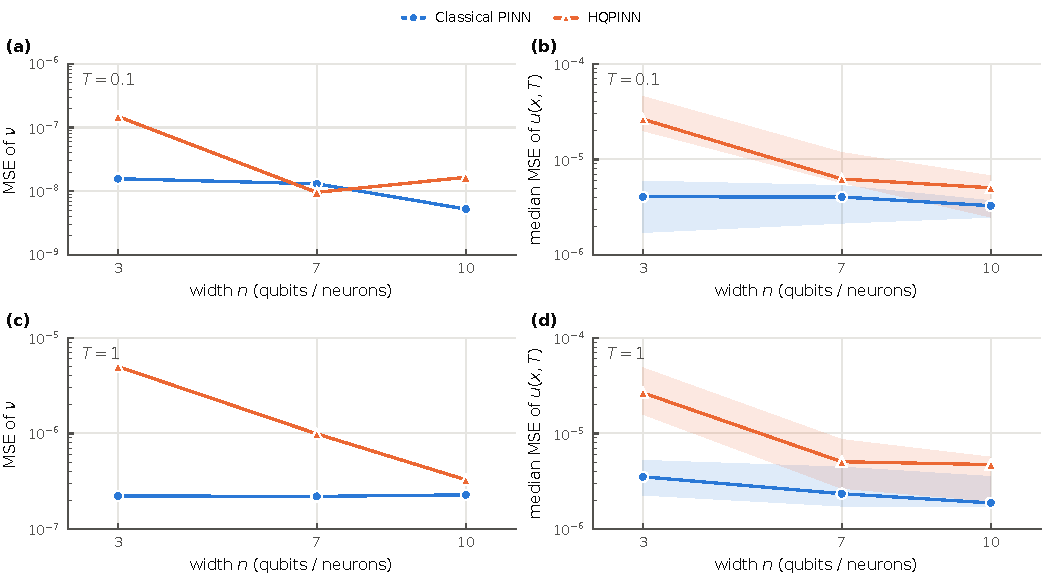
\includegraphics[width=\textwidth]{figC1_inv_long.pdf}
  \caption{\justifying Inverse problem at $K=20\,000$ epochs with the noiseless layer: mean squared error of the learned viscosity, the mean of $(\hat\nu-\nu_{\rm true})^2$ over seeds 0--10, versus the size $n$ (neurons of the classical bottleneck or qubits), for (a) $T=0.1$ and (b) $T=1$. Blue circles, classical PINN; orange triangles, HQPINN with the ideal circuit.}
  \label{fig:invlong}
\end{figure*}


% ---------------------------------------------------------------------
\section{Inverse problem: real hardware}\label{app:iqpu}
% ---------------------------------------------------------------------
\TODO{Nenhuma rodada real do problema inverso foi executada: este ap\^endice descreve o que est\'a pronto e o que falta decidir. Substituir pelos detalhes da rodada quando ela existir, como no Ap\^endice~\ref{app:run}.}

\subsection{Protocol}\label{app:iprot}
The script of the emulated runs also drives a real processor. It uses the machinery of Appendix~\ref{app:hil} (chain search and screening, packed circuit in a runtime \texttt{Session}, chip-averaged surrogate, refit every 10 epochs, final validation on the device). The differences with respect to the forward run are the following. (i) The measured values at the centres also enter the data term. (ii) Each measurement serves 16 AdamW steps, all with the same offsets, so the number of steps does not change the number of jobs. (iii) At $T=1$ the $\Ncol$ points of the initial-condition term are measured in the same job as the centres (20 points per job). (iv) The validation job uses 100 points instead of 200.

\subsection{Proposed cases and cost}\label{app:icost}
The cases listed in the code (\texttt{INVERSE\_QPU\_CASES}) are a proposal: $n=10$, $\Ncol=10$, 110 epochs, seed 0, at $T=0.1$ and $T=1$, the same size and budget as the forward run. Table~\ref{tab:icost} gives the cost estimated from the forward run, assuming the same 8 chains and the same latency of 16~s per epoch. A run at $K=500$ would take about 2.2~h at that latency, above the limit of 2~h per \texttt{Session} set in the script.

\begin{table}[h]
\caption{\justifying Estimated cost of an inverse run on \texttt{ibm\_berlin} ($n=10$, 8 chains, $K=110$, $S=1024$). These are estimates, not measurements: 128 calibration sets, $\lceil\text{points}/8\rceil$ sets per training job, 100 validation sets.}
\label{tab:icost}
\setlength{\tabcolsep}{4pt}
\footnotesize
\begin{ruledtabular}
\begin{tabular}{lcc}
 & $T=0.1$ & $T=1$\\
\colrule
jobs & 112 & 112\\
points per training job & 10 & 20\\
parameter sets & 448 & 558\\
shots & $4.6\times10^5$ & $5.7\times10^5$\\
wall-clock time & $\sim1$~h & $\sim1$~h\\
\end{tabular}
\end{ruledtabular}
\end{table}

\subsection{Open choices}\label{app:iopen}
\TODO{Decidir antes de rodar:
(1) \emph{mitiga\c{c}\~ao:} o padr\~ao do script \'e \texttt{suppress} (TREX, desacoplamento din\^amico e twirling), mas a rodada do problema direto foi sem mitiga\c{c}\~ao e o emulador n\~ao reproduz a mitiga\c{c}\~ao do runtime; para comparar, use \texttt{none};
(2) \emph{QPU:} \texttt{ibm\_berlin} (compara com o direto e com $K=110$) ou \texttt{ibm\_aachen} (compara com $K=500$);
(3) \emph{seed:} fix\'a-la antes de ver o QPU; se for a melhor de um lote no emulador, dizer no texto;
(4) \emph{estat\'istica:} uma rodada s\'o n\~ao se compara com o emulador em $\nu$, porque o $\nu$ final de uma rodada oscila muito; ao menos algumas seeds seriam necess\'arias, sobretudo em $T=1$.}

\end{appendices}

\bibliography{references}

\end{document}
